\documentclass[11pt]{article}
\usepackage[T1]{fontenc}
\usepackage{lmodern}
\usepackage[margin=1in]{geometry}
\usepackage{amsmath,amssymb,amsthm,mathtools}
\usepackage{microtype}
\usepackage{xcolor}
\usepackage{tikz}
\usepackage[colorlinks=true,linkcolor=blue!45!black,citecolor=green!35!black,urlcolor=blue!45!black]{hyperref}
\usepackage{bookmark}
\hypersetup{pdftitle={Full support of the zero-temperature Sherrington--Kirkpatrick order parameter},pdfauthor={OpenAI}}
\pdfglyphtounicode{parenleftbig}{0028 FE01}
\pdfglyphtounicode{parenrightbig}{0029 FE01}
\pdfglyphtounicode{vextendsingle}{20D3}
\pdfglyphtounicode{parenleftbigg}{0028 FE03}
\pdfglyphtounicode{parenrightbigg}{0029 FE03}
\pdfglyphtounicode{bracketleftbigg}{005B FE03}
\pdfglyphtounicode{bracketrightbigg}{005D FE03}
\pdfglyphtounicode{parenleftBigg}{0028 FE04}
\pdfglyphtounicode{parenrightBigg}{0029 FE04}
\pdfglyphtounicode{braceleftBigg}{007B FE04}
\pdfglyphtounicode{bracerightBigg}{007D FE04}
\pdfglyphtounicode{summationtext}{2211 FE01}
\pdfglyphtounicode{integraltext}{222B FE01}
\pdfglyphtounicode{summationdisplay}{2211 FE02}
\pdfglyphtounicode{integraldisplay}{222B FE02}
\pdfglyphtounicode{hatwide}{02C6 FE01}
\pdfglyphtounicode{tildewide}{02DC FE01}
\pdfglyphtounicode{bracketleftBig}{005B FE02}
\pdfglyphtounicode{bracketrightBig}{005D FE02}
\pdfglyphtounicode{radicalbig}{221A FE01}
\pdfglyphtounicode{radicalbigg}{221A FE03}
\pdfglyphtounicode{radicalBigg}{221A FE04}
\pdfglyphtounicode{mapsto}{007C}
\pdfgentounicode=1

\newcommand{\E}{\mathbb E}
\newcommand{\R}{\mathbb R}
\newcommand{\dd}{\mathrm d}
\DeclareMathOperator{\supp}{supp}
\DeclareMathOperator{\Var}{Var}
\newtheorem{theorem}{Theorem}[section]
\newtheorem{lemma}[theorem]{Lemma}
\newtheorem{proposition}[theorem]{Proposition}
\newtheorem{corollary}[theorem]{Corollary}
\theoremstyle{remark}
\newtheorem{remark}[theorem]{Remark}
\numberwithin{equation}{section}
\setlength{\emergencystretch}{2em}
\title{Full support of the zero-temperature\\
Sherrington--Kirkpatrick order parameter}
\author{OpenAI}
\date{September 27, 2026}
\begin{document}
\maketitle
\begin{abstract}
We prove that every admissible integrable minimizer of the zero-temperature
Parisi functional for the pure, zero-field Sherrington--Kirkpatrick model
has full relative Stieltjes support on $[0,1)$. Thus its support has no
gaps at any overlap scale below one. We use the covariance normalization
$\xi(t)=t^2/2$.
\end{abstract}

\section{Introduction}
For independent standard Gaussian variables $J_{ij}$ and spins
$\sigma\in\{-1,1\}^n$, the pure Sherrington--Kirkpatrick (SK) Hamiltonian
with no external field is
\[
 H_n(\sigma)=\frac1{\sqrt n}\sum_{i<j}J_{ij}\sigma_i\sigma_j.
\]
Its ground-state problem asks for the limiting maximum energy per spin.
The Parisi variational formula expresses this value through an order
parameter encoding a hierarchy of overlap scales. Infinitely many
scales need not fill an interval; the question studied here is whether
every scale below one belongs to the zero-temperature support.

We first specify the variational problem, including the convention at the
left endpoint. Let $\mathcal U$ be the set of nonnegative, nondecreasing,
right-continuous functions $\gamma:[0,1)\to[0,\infty)$ satisfying
$\int_0^1\gamma(t)\,\dd t<\infty$. The Stieltjes measure $\mu_\gamma$
on $[0,1)$ is defined by
\[
 \mu_\gamma([0,t])=\gamma(t),\qquad 0\leq t<1.
\]
In particular $\mu_\gamma(\{0\})=\gamma(0)$. It is locally finite,
but need not be a probability measure or have finite total mass.
All support statements below use the relative topology of $[0,1)$.

For $\gamma\in\mathcal U$, define the Parisi value function by
\begin{equation}\label{eq:model-control}
 \Phi_\gamma(t,x)=\sup_{|a|\leq1}\E\left[
 \left|x+B_1-B_t+\int_t^1\gamma(s)a_s\,\dd s\right|
 -\frac12\int_t^1\gamma(s)a_s^2\,\dd s\right].
\end{equation}
Here $B$ is standard Brownian motion and the supremum is over progressively
measurable controls $a_s\in[-1,1]$, adapted to its increments after time
$t$. This is the solution, obtained by monotone-coefficient approximation,
of
\begin{equation}\label{eq:model-pde}
 \Phi_t=-\tfrac12(\Phi_{xx}+\gamma(t)\Phi_x^2),
 \qquad \Phi(1,x)=|x|.
\end{equation}
Section~\ref{sec:regularity} proves the regularity and approximation facts
we use, directly from the heat equation and~\eqref{eq:model-control}.
The functional to be minimized is
\begin{equation}\label{eq:model-functional}
 \mathcal P(\gamma)=\Phi_\gamma(0,0)
                  -\frac12\int_0^1t\gamma(t)\,\dd t.
\end{equation}

This normalization has covariance $\xi(t)=t^2/2$, hence $\xi''=1$.
For two spin configurations with overlap
$R_{12}=n^{-1}\sum_i\sigma_i^1\sigma_i^2$, the covariance is
$\E H_n(\sigma^1)H_n(\sigma^2)=nR_{12}^2/2-1/2$.
Adding an independent centered Gaussian of variance $1/2$, constant
across spin configurations, gives exactly $n\xi(R_{12})$ and leaves
the expected maximum unchanged. The zero-temperature Parisi formula
and its attainment give\footnote{The normalized maximum is a Lipschitz
function of the Gaussian disorder with constant
$\sqrt{(n-1)/(2n^2)}$. Gaussian concentration makes its difference
from its expectation tend to zero in probability. Together with the
almost-sure ground-state limit in the cited formula, this implies
convergence of the expectations to the same constant.}
\begin{equation}\label{eq:model-ground-state}
 P_*:=\lim_{n\to\infty}\frac1n\E\max_\sigma H_n(\sigma)
     =\min_{\gamma\in\mathcal U}\mathcal P(\gamma).
\end{equation}
We use this established formula and existence theorem from
Auffinger and Chen~\cite[Theorem~1 and the proof of Lemma~3]{AC2017}.
The proof of the support assertion itself applies to any minimizer of
the explicitly defined functional~\eqref{eq:model-functional}.

Write $u_\gamma=\Phi_{\gamma,x}$ and define its controlled diffusion by
\begin{equation}\label{eq:model-diffusion}
 \dd X_t=\gamma(t)u_\gamma(t,X_t)\,\dd t+\dd B_t,
 \qquad X_0=0.
\end{equation}
The drift is bounded and Lipschitz in space on every compact time strip;
its absolute value is bounded by the integrable function $\gamma$.
Thus this equation has a unique strong solution up to time one, as proved
in Lemma~\ref{lem:diffusion}.

\begin{theorem}[Full support at zero temperature]\label{thm:full-support}
If $\gamma\in\mathcal U$ minimizes $\mathcal P$, then
\[
 \supp\mu_\gamma=[0,1).
\]
In particular $\gamma(b)>\gamma(a)$ whenever $0\leq a<b<1$.
For the solution of~\eqref{eq:model-diffusion},
\begin{equation}\label{eq:main-consistency}
 \E[u_\gamma(t,X_t)^2]=t,\qquad
 \E[\Phi_{\gamma,xx}(t,X_t)^2]=1,
 \qquad 0\leq t<1.
\end{equation}
\end{theorem}

Chen~\cite[Theorem~1.3]{Chen2026} proves the same full-relative-support
conclusion, together with smooth absolute continuity of the minimizing
Stieltjes measure. The present proof excludes gaps through an explicit
rational coercive identity and an unconditional strict-curvature inequality
on positive constant intervals. Corollary~\ref{cor:smooth-measure}
recovers $\gamma\in C^\infty([0,1))$ and $\gamma(0)=0$ by the
consistency and polynomial-moment argument of
\cite[Proposition~4.6 and Appendix~B.6]{Chen2026}. A fixed-time
approximation by constant intervals then transfers our coercive bound
to the minimizer and gives $\gamma'(t)>0$ for $0<t<1$.
Thus $\mu_\gamma=\gamma'(t)\,\dd t$ has a smooth density which is
strictly positive away from zero. We also develop the scalar martingale
value representation and finite Gaussian coefficients in
Section~\ref{sec:consequences}, and apply the optimization theorem of
El Alaoui, Montanari, and Sellke in Corollary~\ref{cor:algorithm}.

Zero external field is used in the evenness of $\Phi$ and the
initial condition $X_0=0$; the constant value of $\xi''$ is used in the
curvature identities. Neither a nonzero-field extension nor an extension
to a general mixed-spin covariance is implicit in the statement.

\subsection{Prior work and the distinction between support assertions}
Sherrington and Kirkpatrick introduced the infinite-range Gaussian Ising
spin-glass model~\cite{SK1975}. Parisi proposed a hierarchy of
replica-symmetry breaking described by a functional order
parameter~\cite{Parisi1979}; its interpretation through overlaps was
developed subsequently~\cite{Parisi1983}. Guerra established the
interpolation bound for the Parisi variational expression~\cite{Guerra2003},
and Talagrand proved the Parisi formula for the SK free energy at every
positive temperature~\cite{Talagrand2006}. Identifying the support of
the minimizing order parameter is a separate question from proving
that variational formula.

The zero-temperature variational problem is part of the rigorous Parisi
theory developed by Auffinger and Chen~\cite{AC2017}. The control
formulation has antecedents in the Brownian variational representation
of Bou\'e and Dupuis~\cite{BD1998} and the diffusion-control representation
of the Parisi equation in Bovier and Klimovsky~\cite[Section~6.2]{BK2009}.
Auffinger and Chen~\cite{AC2015} and Jagannath and Tobasco~\cite{JT2016}
developed stochastic-control, strict-convexity, and gradient-martingale
arguments for this equation. Chen, Handschy, and
Lerman~\cite[Propositions~2--4, Theorems~4--5, and Lemma~3]{CHL2018}
give zero-temperature regularity, control, uniqueness, and variation
interfaces. We prove the analytic and variational facts needed here,
including global-in-space derivative convergence on compact time strips,
rather than presume that a smooth-terminal statement applies at the
terminal cusp $|x|$.

Auffinger, Chen, and Zeng proved that the zero-temperature SK order
parameter has infinitely many support points~\cite[Theorem~1]{ACZ2017}.
They also recorded the exclusion of a terminal constant interval
\cite[Remark~7]{ACZ2017}; Section~\ref{sec:variation} supplies a detailed
boundary-layer proof of that endpoint fact. Infinite support and absence
of a terminal plateau do not exclude an interior gap. The main issue
here is the elimination of every such gap.

At positive temperature, Zhou~\cite[Theorem~1]{Zhou2026} established
an interval-support result near the critical temperature, and
Lopatto~\cite[Theorem~1.1]{Lopatto2026} established full interval support
throughout the zero-field SK low-temperature phase. Lopatto's proof
propagates inequalities for Cole--Hopf profiles and a transformed
diffusion density before applying a constant-interval crossing argument
\cite[Sections~3, 7--9]{Lopatto2026}. Chen's zero-temperature analysis
also uses transformed-density inequalities and smooth-terminal
approximation~\cite[Propositions~3.7 and 3.11]{Chen2026}.
The crossing conclusions in \cite[Proposition~9.1]{Lopatto2026} and
\cite[Proposition~4.2]{Chen2026} are conditional: if the second derivative
of the gradient's second moment vanishes at a point of a positive constant
interval, its third derivative is positive at that point. Our rational identity instead bounds
that third derivative below by a strictly positive quantity throughout
each such interval. The argument is carried out directly at zero
temperature; interval support alone does not in general pass through
weak limits of measures.

The variational contact conditions have precedents in both the
positive-temperature analysis of Jagannath and
Tobasco~\cite[Proposition~1.1, Lemma~3.2, and Corollaries~3.6 and 3.10]{JT2017}
and the zero-temperature analysis of Chen, Handschy, and
Lerman~\cite[Propositions~3--4]{CHL2018}. In the present setting one may
add or remove Stieltjes mass without a probability normalization constraint.
This gives a contact potential which is nonnegative and vanishes on the
support, a fact we derive explicitly.
Once consistency is saturated at every time, differentiating polynomial
moments yields regularity of the order parameter. This method appears in
Auffinger and Chen~\cite[Lemma~2 and the proof of Theorem~2(ii)]{ACProperties2015}
and in the zero-temperature form of Chen~\cite[Appendix~B.6]{Chen2026}.

The scalar consequences in Section~\ref{sec:consequences} follow the
incremental approximate-message-passing methodology of
Montanari~\cite{Montanari2019} and El Alaoui, Montanari, and
Sellke~\cite{EAMS2021}: a Hessian-weighted gradient martingale determines
normalized Euler increments and the limiting value. We prove the needed
scalar statements directly. The finite-disorder algorithm is supplied
separately by the theorem of El Alaoui, Montanari, and
Sellke~\cite[Theorem~3 and Corollary~2.2 of the cited preprint]{EAMS2021}:
full support verifies its strictly increasing minimizer hypothesis.
Corollary~\ref{cor:algorithm} spells out the Gaussian input normalization
and the resulting $C(\epsilon)n^2$ real-arithmetic operation count.

\subsection{Proof structure}
The argument has an analytic part and a variational part.
Section~\ref{sec:regularity} first constructs the diffusion and proves
the compact-strip estimates needed to approximate integrable order
parameters. Set $q(t)=\E u_\gamma(t,X_t)^2$. The gradient-martingale identity gives
$q'(t)=\E\Phi_{\gamma,xx}(t,X_t)^2$. At a minimizer, the first variation
shows that
\[
 G(s)=\int_s^1(q(t)-t)\,\dd t
\]
is nonnegative and vanishes on $\supp\mu_\gamma$. At an interior support
point this implies $q(t)=t$ and $q'(t)\leq1$.
On a hypothetical interior gap $(a,b)$ with $\gamma=c>0$, the endpoint
conditions give $q(a)=a$, $q(b)=b$, and $q'(a),q'(b)\leq1$.
If $q'$ is strictly convex there, it lies below its endpoint chord and
hence below $1$ inside. Integrating gives $q(b)-q(a)<b-a$, contradicting
contact at the endpoints, as illustrated in Figure~\ref{fig:gap-convexity}.
\begin{figure}[tbp]
\centering
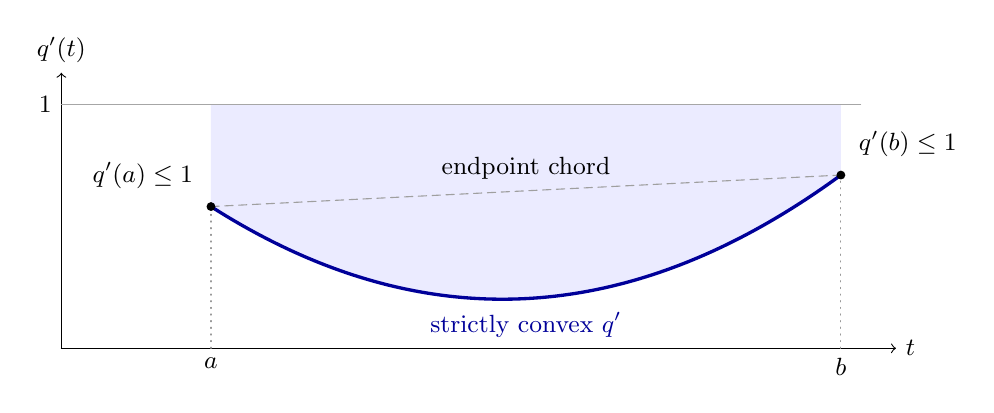
\begin{tikzpicture}[x=1cm,y=1cm,font=\small,line cap=round]
  \fill[blue!8] (0,3.1) -- (8,3.1) -- (8,2.2)
     .. controls (5.3333,.25) and (2.6667,.10) .. (0,1.8) -- cycle;
  \draw[->] (-1.9,0) -- (8.7,0) node[right] {$t$};
  \draw[->] (-1.9,0) -- (-1.9,3.5) node[above] {$q'(t)$};
  \draw[gray!70] (-1.9,3.1) -- (8.25,3.1);
  \node[left] at (-1.9,3.1) {$1$};
  \draw[densely dashed,gray!75] (0,1.8) -- (8,2.2)
    node[midway,above=3pt,text=black,fill=blue!8,inner sep=1pt]
       {endpoint chord};
  \draw[very thick,blue!60!black] (0,1.8)
    .. controls (2.6667,.10) and (5.3333,.25) .. (8,2.2);
  \draw[dotted,gray!80] (0,0) -- (0,1.8);
  \draw[dotted,gray!80] (8,0) -- (8,2.2);
  \fill (0,1.8) circle (1.6pt);
  \fill (8,2.2) circle (1.6pt);
  \node[below] at (0,0) {$a$};
  \node[below] at (8,0) {$b$};
  \node[above left=3pt] at (0,1.8) {$q'(a)\le1$};
  \node[above right=3pt] at (8,2.2) {$q'(b)\le1$};
  \node[below,blue!60!black] at (4,.58) {strictly convex $q'$};
\end{tikzpicture}
\caption{The contradiction on a hypothetical support gap with
$\gamma=c>0$. Strict convexity puts $q'$ below its endpoint chord,
which is at most $1$. The shaded deficit is positive, whereas contact
at both endpoints requires $\int_a^bq'(t)\,\dd t=q(b)-q(a)=b-a$.
The endpoint derivatives need not equal $1$.}
\label{fig:gap-convexity}
\end{figure}


The main work is to establish this strict convexity without assuming
support properties. For a positive constant coefficient $c$, put
$r=c\Phi_x$, $v=r_x$, $w=r_{xx}$, and $z=r_{xxx}$.
Direct differentiation along the diffusion yields
\[
 q'''(t)=c^{-2}\E[z^2-12vw^2+6v^4](t,X_t).
\]
The expression inside this expectation has a negative term and is not
controlled pointwise by convexity of $\Phi$ alone.
Sections~\ref{shape:section} and~\ref{cert:section} overcome this
obstacle. For positive finite-step coefficients with smooth terminal
data, let $f(t,\cdot)$ be the density of $X_t$. The factorization
$f=e^{c\Phi}g$ gives a forward heat equation for $g$ between jumps.
We propagate backward shape inequalities for $r$ and forward inequalities
for the score $s=-\partial_x\log g$, including a comparison of $s/r$.
These signs make an exact rational polynomial identity nonnegative
after one spatial integration by parts, retaining the lower bound
$10^{-3}\E v^4$.

Section~\ref{sec:curvature} transfers only this integrated inequality
to an arbitrary integrable coefficient; it does not require convergence
of the auxiliary density scores or their ratios. The zero-coefficient
case follows separately from the heat equation. Section~\ref{sec:variation}
then excludes interior, initial, and terminal gaps. With $q(t)=t$ at
every time, the Hessian It\^o identity expresses $\gamma$ as a
quotient of continuous derivative moments. Differentiating polynomial
moments simultaneously bootstraps this formula to smoothness.
To obtain $\gamma'(t)>0$ at a fixed $t>0$, we approximate $\gamma$ by
coefficients which equal $\gamma(t)$ on shrinking intervals around $t$.
The integrated coercive inequality passes to the limit at that fixed
time and becomes a strictly positive lower bound for $\gamma'(t)$.
Finally, Section~\ref{sec:consequences} derives a martingale formula
for $P_*$ and a finite Gaussian approximation, then verifies the
hypothesis and normalization of the existing optimization theorem.

\section{Integrable coefficients and the controlled diffusion}
\label{sec:regularity}

The sign inequalities will first be proved for finite step functions.  We
therefore need estimates which survive approximation of an arbitrary
$\gamma\in\mathcal U$, including coefficients which diverge at time one.
All estimates in this section are on strips ending strictly before one.
The control and heat-semigroup methods follow the Parisi PDE framework of
Auffinger and Chen~\cite{AC2015}, Jagannath and Tobasco~\cite{JT2016},
and the zero-temperature treatment of Chen, Handschy, and
Lerman~\cite[Proposition~2 and Theorem~5]{CHL2018}.
We include the proofs to make the approximation uniformity explicit.
We retain the notation $u_\gamma=\partial_x\Phi_\gamma$ from the model
definition, and write $P_t$ for the heat semigroup with variance $t$.

\begin{lemma}[Compact-strip regularity and stability]
\label{lem:regularity}
For every $\gamma\in\mathcal U$, the function $\Phi_\gamma$ is even,
convex, and one-Lipschitz in its spatial variable.  It satisfies
\begin{equation}
 |x|\leq\Phi_\gamma(t,x)
 \leq |x|+\sqrt{\frac{2(1-t)}\pi}
               +\frac12\int_t^1\gamma(s)\,\dd s.
 \label{eq:terminal-uniform}
\end{equation}
For each integer $k\geq1$ and $T<1$, the derivative
$\partial_x^k\Phi_\gamma$ is bounded and jointly continuous on
$[0,T]\times\R$.  These bounds are uniform when the coefficients have
uniformly bounded $L^1(0,1)$ norms.  The derivatives are locally
absolutely continuous in time and satisfy the spatially differentiated
Parisi equation for almost every time.

If $\gamma_n\to\gamma$ in $L^1(0,1)$, then, for every $k\geq1$ and
$T<1$,
\begin{equation}
 \sup_{[0,T]\times\R}
 |\partial_x^k\Phi_{\gamma_n}-\partial_x^k\Phi_\gamma|
 \longrightarrow0.
 \label{eq:derivative-convergence}
\end{equation}
The same conclusion holds when each $\gamma_n$ is a finite step
function and its terminal datum is
$M_n^{-1}\log(2\cosh(M_nx))$, where $M_n\to\infty$.
\end{lemma}

\begin{proof}
For a nonnegative finite step coefficient and a smooth even convex
one-Lipschitz terminal datum $\psi$, backward evolution across an
interval with coefficient $c$ is
\begin{equation}
 \Phi(t,x)=
 \begin{cases}
 c^{-1}\log P_{b-t}(e^{c\Phi(b,\cdot)})(x),&c>0,\\
 P_{b-t}\Phi(b,\cdot)(x),&c=0.
 \end{cases}
 \label{eq:constant-heat}
\end{equation}
These formulas preserve evenness, convexity, and the one-Lipschitz
bound.  Convexity in the first case follows either from H\"older's
inequality applied after a spatial translation, or by differentiating
the logarithm: its second derivative is the tilted mean of the old
second derivative plus $c$ times the tilted variance of the old first
derivative.  The first derivative is a tilted mean of the old first
derivative.  The assertions in the case $c=0$ follow directly from
convolution.

For these step solutions, It\^o's formula and completion of the square
give the control representation
\begin{equation}
 \Phi(t,x)=\sup_{|a|\leq1}\E\left[
 \psi\left(x+B_1-B_t+\int_t^1\gamma(s)a_s\,\dd s\right)
 -\frac12\int_t^1\gamma(s)a_s^2\,\dd s\right].
 \label{eq:control-representation}
\end{equation}
The supremum is over progressively measurable controls.  Indeed, the
drift of $\Phi(s,Y_s)-\frac12\int_t^s\gamma a^2$ is
$-\gamma(a-u_\gamma)^2/2$ when
$\dd Y_s=\gamma(s)a_s\,\dd s+\dd B_s$.  Equality is attained by
$a_s=u_\gamma(s,Y_s)$; for the smooth finite-step problem the feedback
equation has a unique strong solution.  Consequently two such
solutions obey
\begin{equation}
 \|\Phi_{\gamma,\psi}-\Phi_{\widetilde\gamma,\widetilde\psi}
       \|_\infty
 \leq\|\psi-\widetilde\psi\|_\infty
             +\frac32\|\gamma-\widetilde\gamma\|_1.
 \label{eq:value-stability}
\end{equation}
Here the supremum is over the whole time-space domain, even though the
individual functions grow linearly.  The bound follows by using the
same controls on both sides of \eqref{eq:control-representation}.

Nonnegative nondecreasing finite step functions are dense in
$\mathcal U$ for the $L^1$ norm.  For example, truncate at a time
increasing to one, approximate the resulting bounded monotone
function by monotone step functions, and then let the truncation time
tend to one.  Since
$0\leq M^{-1}\log(2\cosh(Mx))-|x|\leq M^{-1}\log2$,
\eqref{eq:value-stability} defines a unique uniform limit, with control
representation \eqref{eq:control-representation} and terminal datum
$|x|$.  This agrees with the Parisi solution in the model definition.
All the asserted shape properties pass to the limit.  The zero control
and Jensen's inequality give the lower bound in
\eqref{eq:terminal-uniform}.  For the upper bound use the triangle
inequality and $|a|-a^2/2\leq1/2$ in the control representation.

We give the smoothing estimates explicitly.  This also establishes
the uniformity needed below.  On any strip $[0,b]$ with $b<1$,
monotonicity gives
\begin{equation}
 \gamma(t)\leq\frac{\|\gamma\|_1}{1-b},\qquad 0\leq t\leq b.
 \label{eq:local-coefficient-bound}
\end{equation}
Thus all coefficients in an $L^1$-bounded family have a common bound
$\Gamma$ there.  Work first with the smooth-terminal step solutions
and put $U=\Phi_x$.  Differentiation of the mild equation gives
\begin{equation}
 U(t)=P_{b-t}U(b)
       +\int_t^b\gamma(s)P_{s-t}[U(s)U_x(s)]\,\dd s.
 \label{eq:burgers-mild}
\end{equation}
We always have $\|U\|_\infty\leq1$, independently of its terminal
smoothing.  The heat-kernel estimate
$\|\partial_xP_h f\|_\infty\leq C h^{-1/2}\|f\|_\infty$
implies
\begin{equation}
 \|U_x(t)\|_\infty
 \leq \frac{C}{\sqrt{b-t}}
       +C\Gamma\int_t^b
                  \frac{\|U_x(s)\|_\infty}{\sqrt{s-t}}\,\dd s.
 \label{eq:fractional-bound}
\end{equation}
The constants do not involve derivatives of the terminal datum.

For completeness, the integral inequality in
\eqref{eq:fractional-bound} gives a uniform bound away from $b$.
The convolution of $h^{-1/2}$ with itself equals $\pi$.
Substituting the inequality once into its integral therefore reduces
it to an ordinary backward Gronwall inequality, with forcing bounded
by a constant times $1+(b-t)^{-1/2}$.  That forcing is integrable.
The resulting estimate is uniform on every smaller strip.

The same argument bounds all higher derivatives.  Suppose that
derivatives of $U$ through order $m-1$ are already bounded on a
slightly larger strip.  Differentiate \eqref{eq:burgers-mild} $m$
times, placing one derivative on the heat kernel and the other
$m-1$ on $UU_x$.  Its highest-order term is
$U\partial_x^mU$; every remaining product involves derivatives of
orders at most $m-1$.  The initial term is bounded by
$C(b-t)^{-1/2}\|\partial_x^{m-1}U(b)\|_\infty$.
Thus the same integral inequality applies to
$\|\partial_x^mU(t)\|_\infty$, with an additional bounded forcing.
Choose successively smaller strip endpoints in this induction.
For every fixed $m$ this proves the asserted bound, uniformly for
the approximants.

Uniform convergence of the functions now gives convergence of all
their spatial derivatives without a separate singular-kernel
comparison.  If a bounded $C^2$ function $F$ on $\R$ has bounded
second derivative, Taylor's formula gives, for every $h>0$,
\begin{equation}
 \|F'\|_\infty\leq
 \frac{2\|F\|_\infty}{h}
       +\frac h2\|F''\|_\infty.
 \label{eq:interpolation}
\end{equation}
Apply this to a difference of two approximating solutions, uniformly
on a fixed smaller strip.  The uniform second-derivative bound and
uniform convergence imply convergence of the first derivatives.
Apply \eqref{eq:interpolation} successively to the differences of
the first, second, and later derivatives; the next two derivative
bounds are available at every stage.  This proves uniform convergence
of every positive spatial derivative.  Their limits are the spatial
derivatives of the limiting function, by the fundamental theorem of
calculus.  Since the approximating derivatives are jointly continuous,
so are their uniform limits.

The argument applies also to an arbitrary $L^1$-convergent sequence in
$\mathcal U$: first obtain these bounds for each member by step
approximation, then use \eqref{eq:value-stability}, the uniform local
coefficient bound \eqref{eq:local-coefficient-bound}, and
\eqref{eq:interpolation}.  Finally pass to the limit in the integral
form of the differentiated equation on each compact strip.
All its spatial factors converge uniformly, and its coefficient
converges in $L^1$.  This proves local absolute continuity in time and
the asserted almost-everywhere equations.
\end{proof}

\begin{lemma}[Diffusion and square-martingale identity]
\label{lem:diffusion}
For $\gamma\in\mathcal U$, the equation
\begin{equation}
 \dd X_t=\gamma(t)u_\gamma(t,X_t)\,\dd t+\dd B_t,
 \qquad X_0=0,
 \label{eq:controlled-diffusion}
\end{equation}
has a unique strong solution on $[0,1]$.  On every strip $[0,T]$ with $T<1$,
\begin{equation}
 u_\gamma(t,X_t)=\int_0^t
                \Phi_{\gamma,xx}(s,X_s)\,\dd B_s.
 \label{eq:gradient-martingale}
\end{equation}
In particular, $q(t)=\E[u_\gamma(t,X_t)^2]$ belongs to $C^1[0,1)$,
$q(0)=0$, and
\begin{equation}
 q'(t)=\E[\Phi_{\gamma,xx}(t,X_t)^2].
 \label{eq:qprime}
\end{equation}
Under the approximations in Lemma~\ref{lem:regularity}, the coupled
diffusions converge uniformly on compact time strips, and $q_n$ and
$q_n'$ converge uniformly there.
\end{lemma}

\begin{proof}
The drift is measurable in time, bounded by $\gamma(t)$, and globally
Lipschitz in space on every compact time strip by
Lemma~\ref{lem:regularity}.  Picard iteration gives a unique strong
solution there.  These solutions agree on overlaps and extend to
time one because $\int_0^1\gamma<\infty$ and Brownian paths are
continuous.

For clarity, convergence needs no moment estimate for the
approximating paths.  Couple them using the same Brownian motion.
The drift difference is bounded by a common spatial Lipschitz
constant times $|X_n-X|$, plus
$|\gamma_n-\gamma|+\gamma_n\|u_n-u_\gamma\|_\infty$.
Gronwall's inequality gives a deterministic bound for
$\sup_{t\leq T}|X_n(t)-X(t)|$ tending to zero.  For step coefficients
and smooth terminal data, It\^o's formula on each step cancels the
drift of $u_n(t,X_n(t))$.  The step-boundary values agree.  Passing to
the limit in the stochastic integral by its $L^2$ isometry proves
\eqref{eq:gradient-martingale}.  Its initial value is zero by evenness.
The same isometry gives
$q(t)=\int_0^t\E[\Phi_{\gamma,xx}(s,X_s)^2]\,\dd s$.
The integrand is continuous by joint continuity, boundedness on
compact strips, and continuity of $X$.  This proves
\eqref{eq:qprime} and the stated convergence assertions.
\end{proof}

\begin{lemma}[Transfer on a constant interval]
\label{lem:constant-transfer}
Suppose $\gamma=c$ on an open interval $I\subset(0,1)$.
If $c>0$, every point of $I$ has a neighborhood on which one may
choose positive, bounded, nondecreasing finite step approximants
equal to $c$, with smooth terminal data and
$M_n\geq\|\gamma_n\|_\infty$.  At each time in this neighborhood,
all spatial derivatives and the corresponding diffusion
expectations of bounded polynomials in those derivatives converge.
Moreover, $\Phi_{\gamma,xx}>0$ throughout $I\times\R$.

For $c>0$, set $r=c\Phi_x$, $v=r_x$, $w=r_{xx}$, and $z=r_{xxx}$.
Then, within $I$,
\begin{align}
 (q')'(t)&=c^{-2}\E[w(t,X_t)^2-2v(t,X_t)^3],
 \label{eq:first-curvature}\\
 (q')''(t)&=c^{-2}\E[z(t,X_t)^2-12v(t,X_t)w(t,X_t)^2
                                      +6v(t,X_t)^4].
 \label{eq:second-curvature}
\end{align}
For $c=0$, $q'$ is strictly increasing on $I$.
\end{lemma}

\begin{proof}
To preserve a positive plateau, truncate and discretize the
coefficient separately to the left and right of a closed subinterval
of $I$, retain the value $c$ on that subinterval, and impose a
positive lower cutoff tending to zero and smaller than $c$.
All choices are monotone and converge in $L^1$.  Increase the terminal
smoothing parameter beyond the finite step bound.  The convergence
claims then follow from Lemmas~\ref{lem:regularity} and
\ref{lem:diffusion}.  The products involved are uniformly bounded,
and the spatial derivative bounds also give uniform continuity for
evaluating them on the coupled paths.

For strict positivity, choose $b\in I$ later than the time in
question and use \eqref{eq:constant-heat}.  The function
$h=\Phi_\gamma(b,\cdot)$ is smooth, convex, even, and differs from
$|x|$ by a bounded function.  Its derivative is therefore not constant.
Twice differentiating the logarithm in \eqref{eq:constant-heat}
gives
\[
 \Phi_{xx}(t,x)=\E_{t,x}^{\rm tilt}[h'']
                     +c\operatorname{Var}_{t,x}^{\rm tilt}(h').
\]
The tilted Gaussian law has a strictly positive density everywhere.
The variance is strictly positive and the first term is nonnegative.

Inside $I$ all functions are smooth in time as well as space, by
the heat formula.  Along $X$, the drifts of $r$, $v$, and $w$ are
respectively $0$, $-v^2$, and $-3vw$, and their diffusion coefficients
are $v$, $w$, and $z$.  These identities follow by differentiating
$r_t=-r_{xx}/2-rr_x$.  It\^o's formula for $v^2$ and then for
$w^2-2v^3$, with \eqref{eq:qprime}, proves
\eqref{eq:first-curvature}--\eqref{eq:second-curvature}.
All differentiations under the expectation are justified by the
bounded higher spatial derivatives on smaller intervals.

If $c=0$, the same argument gives
\[
 (q')'(t)=\E[\Phi_{xxx}(t,X_t)^2]>0.
\]
To see strictness, start the drift-free interval at any earlier
time in $I$.  Its Gaussian transition kernel implies that $X_t$ has
a strictly positive density on $\R$.  The function
$\Phi_{xxx}(t,\cdot)$ cannot vanish identically: otherwise
$\Phi(t,\cdot)$ would be an even quadratic polynomial, whereas it
is one-Lipschitz and differs from $|x|$ by a bounded function.
\end{proof}

\section{Shape inequalities for finite step functions}
\label{shape:section}

On a positive constant interval, the curvature formula
\eqref{eq:second-curvature} contains the indefinite expression
$z^2-12vw^2+6v^4$.  The next section will make its expectation positive
by adding a spatial derivative of zero expectation.  Our task here is to
prove the shape inequalities that make this possible: we compare the
backward drift with a logarithmic derivative of the forward density.

We work with a fixed positive finite step coefficient and a smooth
terminal condition.  The estimates in this section may depend on these
fixed data.  Section~\ref{sec:curvature} will pass only the resulting
integrated inequality to general coefficients, using
Lemma~\ref{lem:regularity}.

Fix a partition $0=t_0<t_1<\cdots<t_N=1$, constants
$0<c_1\le\cdots\le c_N\le M$, and
$\gamma(t)=c_i$ on $[t_{i-1},t_i)$.  Let $\Phi$ solve
\[
 \Phi_t=-\frac12(\Phi_{xx}+\gamma\Phi_x^2),
 \qquad \Phi(1,x)=M^{-1}\log(2\cosh(Mx)).
\]
On a step where $\gamma=c$, put
\[
 l=c\Phi,\qquad r=l_x,\qquad v=r_x,
 \qquad w=r_{xx},\qquad z=r_{xxx}.
\]
Spatial derivatives of $\Phi$ agree across step boundaries; those of $l$
are rescaled with $c$.  Within a step, $h=e^l$ satisfies
$h_t=-\tfrac12h_{xx}$.  In backward time $\tau$ this gives
\begin{equation}\label{shape:backward-r}
 r_\tau=\frac12r_{xx}+rr_x.
\end{equation}
Let $X_0=0$ and $\dd X_t=r(t,X_t)\dd t+\dd B_t$.  The drift is bounded
and spatially Lipschitz for these fixed data.  Its density at positive times
will be denoted by $f(t,x)$.  Factor it as
\[
 f=e^l g,\qquad s=-\partial_x\log g.
\]
The factor $e^l$ contains the backward solution.  The remaining factor
$g$ evolves by the forward heat equation within each step.  Indeed, the
transition density from time $a$ to time $t$ in the same step is
\[
 p_{t-a}(x-y)\frac{h(t,x)}{h(a,y)},\qquad
 p_u(x)=(2\pi u)^{-1/2}e^{-x^2/(2u)}.
\]
It integrates to one because $h(a,\cdot)=P_{t-a}h(t,\cdot)$, and
differentiation verifies the forward equation with drift $r=h_x/h$.
Consequently $g_t=\tfrac12g_{xx}$.  On the first step,
$g(t,x)=p_t(x)/h(0,0)$, so $s=x/t$.  At a forward jump
$c_+-c_-=\delta\ge0$, continuity of $f$ gives
\begin{equation}\label{tail:g-jump}
 g_+=g_-e^{-\delta\Phi}.
\end{equation}
In particular $g$ is positive and even, and $s$ is odd.

The comparison we need has three parts.  On the positive half-line the
drift $r$ is increasing and concave; its relative backward-time change
$r_\tau/r$ is nonpositive and nondecreasing in $x$.  The score $s$ is also
increasing and concave, and its ratio to $r$ is nondecreasing in $x$.
Lemmas~\ref{shape:backward} and~\ref{shape:forward} state these claims
precisely.  We first record the boundary estimates needed in their proofs.

\subsection{Boundary estimates and comparison}

A differentiated exponential error means that, for each fixed finite
derivative order, the error and all its derivatives up to that order
are $O(e^{-\kappa x})$ as $x\to+\infty$, for some $\kappa>0$.
Constants may change with the derivative order.

\begin{lemma}[Differentiated tails]\label{tail:class}
On each closed backward step, uniformly in its time coordinate,
\begin{equation}\label{tail:backward}
 l(t,x)=cx+C(t)+O(e^{-\kappa x})\qquad(x\to+\infty)
\end{equation}
with differentiated exponential error.  The functions are even, so the
negative tail is determined by symmetry.

For the forward heat factor $g$, on every closed forward step with
time bounded away from zero,
\begin{equation}\label{tail:forward}
 g(t,x)=\exp\left(-\frac{x^2}{2t}+\beta(t)x+C_0(t)\right)
                 (1+O(e^{-\kappa x}))\qquad(x\to+\infty),
\end{equation}
with differentiated relative error.  In particular,
\begin{equation}\label{tail:score}
 s(t,x)=\frac{x}{t}-\beta(t)+O(e^{-\kappa x}),\qquad
 s_x(t,x)=\frac1t+O(e^{-\kappa x}),\qquad
 s_{xx}(t,x)=O(e^{-\kappa x}).
\end{equation}
The assertions include one-sided values at every step boundary.
\end{lemma}

The proof uses only Gaussian convolution and the finite-step jump rules;
none of the shape inequalities proved below enters it.

\begin{proof}
Here is a Gaussian estimate that also controls differentiation.  Suppose
$q\in C^m(\mathbb R)$ satisfies, for $0\le j\le m$,
\[
 |q^{(j)}(y)|\le A e^{-\kappa y}\quad(y\ge0),\qquad
 |q^{(j)}(y)|\le A e^{K|y|}\quad(y<0).
\]
For $Y_x=\lambda x+b+\sqrt V Z$, where $Z$ is standard normal,
$0<\lambda_*\le\lambda\le\lambda^*$, $|b|\le B$, and $0\le V\le V_*$,
\begin{equation}\label{tail:gaussian-estimate}
 \partial_x^j\mathbb E q(Y_x)
       =\lambda^j\mathbb E q^{(j)}(Y_x)=O(e^{-\kappa' x})
       \qquad(0\le j\le m)
\end{equation}
uniformly in these parameters, for some $\kappa'>0$.
Indeed, write $\mu=\lambda x+b$ and take $x$ large enough that $\mu>0$.
On $Y_x\ge\mu/2$, use $Ae^{-\kappa\mu/2}$.  On its complement,
the global bound $|q^{(j)}(y)|\le A e^{K|y|}$, Cauchy--Schwarz, and
$\mathbb P(Y_x<\mu/2)\le e^{-\mu^2/(8V_*)}$ give a bound
$C\exp(K\mu-\mu^2/(16V_*))$.  This is smaller than an exponential
in $x$; the case $V=0$ is immediate.  Exponential integrability of the
Gaussian justifies differentiation under the expectation.  Adjusting the
constant covers the remaining bounded range of $x$.

For backward evolution, suppose an even starting function $l_0$ has
$l_0(x)=cx+C+\rho(x)$ with differentiated exponential error.  Set
$q(y)=e^{l_0(y)-cy-C}-1$.  This $q$ obeys the hypotheses above: the
positive tail follows by differentiating the exponential, and evenness of
$l_0$ gives at most exponential growth for $q$ and its derivatives on the
negative tail.  Gaussian tilting gives
\[
 P_\tau(e^{l_0})(x)
 =e^{cx+C+c^2\tau/2}
   \left(1+\mathbb E q(x+c\tau+\sqrt\tau Z)\right).
\]
Apply \eqref{tail:gaussian-estimate} uniformly for bounded $\tau$ and take
the logarithm.  Its relative error tends uniformly to zero, so differentiating
$\log(1+\cdot)$ proves \eqref{tail:backward} with all the stated derivatives.
The initial condition starts this induction since, for $x>0$,
\[
 \frac cM\log(2\cosh Mx)
       =cx+\frac cM\log(1+e^{-2Mx}).
\]
At a backward boundary, $l$ is multiplied by $c_-/c_+>0$, which
preserves the required tail class.  Finite induction proves the first claim.

Suppose at a positive time $a$ that
$g(a,y)=e^{-y^2/(2a)+\beta y+C}(1+q(y))$ has the required tail class.
Evenness of $g$ implies the same exponential-growth bound for the
derivatives of $q$ on the negative tail.  Completing the square gives
\begin{align*}
 P_hg(a,\cdot)(x)
 &=\sqrt{\frac a{a+h}}\,
   \exp\left(-\frac{x^2}{2(a+h)}
      +\frac{a\beta}{a+h}x+C+\frac{\beta^2ah}{2(a+h)}\right)\\
 &\quad\times
   \left(1+\mathbb E q\left(
        \frac a{a+h}x+\frac{\beta ah}{a+h}
           +\sqrt{\frac{ah}{a+h}}Z\right)\right).
\end{align*}
On a fixed interval $0\le h\le H$, the coefficient of $x$ in the
Gaussian mean is at least $a/(a+H)>0$.  Thus
\eqref{tail:gaussian-estimate} proves closure, uniformly including $h=0$.
At a jump, write $\Phi=x+D+\rho$ on the positive tail.  Formula
\eqref{tail:g-jump} replaces $(\beta,C)$ by
$(\beta-\delta,C-\delta D)$ and replaces $1+q$ by
$(1+q)e^{-\delta\rho}$, preserving the differentiated relative error.
Finite induction proves \eqref{tail:forward}.  Logarithmic differentiation
then gives \eqref{tail:score}.
\end{proof}



We will use the following elementary form of comparison.  If on a compact
space-time cylinder
\[
 u_t-\tfrac12u_{xx}-b u_x-c u\ge0,\qquad c\le C,
\]
and $u\ge0$ initially while $u\ge-\varepsilon$ on the lateral boundary,
then
\begin{equation}\label{shape:barrier}
 u(t,x)\ge-\varepsilon e^{(\max(C,0)+1)(t-t_0)}.
\end{equation}
To see this, add the positive exponential on the right to $u$ and multiply
by $e^{-(\max(C,0)+1)(t-t_0)}$.  The resulting zeroth-order coefficient
is at most $-1$.  A negative space-time minimum, which cannot be on the
parabolic boundary, has nonpositive time derivative, zero spatial gradient,
and nonnegative second spatial derivative, contradicting its differential
inequality.  The same proof applies in a ball in $\mathbb R^d$ with
$\tfrac12\Delta$ in place of $\tfrac12\partial_{xx}$.
In particular, to exhaust the line or half-line it suffices that the
lateral boundary errors tend uniformly to zero and that $C$ is independent
of the truncation.  No uniform bound on the first-order coefficient $b$
over the exhausting cylinders is needed.

\subsection{Backward shape inequalities}

\begin{lemma}[Backward shapes]\label{shape:backward}
For the fixed step data above, $r$ is odd and $v>0$.  On $x>0$,
\begin{equation}\label{shape:backward-signs}
 w\le0,\qquad
 H:=\frac{r_\tau}{r}=\frac{w}{2r}+v\le0,
 \qquad H_x\ge0.
\end{equation}
The quotient defining $H$ extends smoothly and evenly at zero.
\end{lemma}

\begin{proof}
Evenness is preserved by both heat evolution and rescaling.  If $l_0''>0$,
the logarithm of its heat evolution obeys
\[
 \partial_{xx}\log P_\tau e^{l_0}(x)
 =\mathbb E_\nu l_0''(Y)
     +\operatorname{Var}_\nu(l_0'(Y))>0,
\]
where $\nu$ is the Gaussian law of $Y=x+\sqrt\tau Z$ tilted by
$e^{l_0(Y)}$; at $\tau=0$ use $l_0''(x)>0$ directly.  Since the terminal
second derivative is $cM\operatorname{sech}^2(Mx)>0$ and backward
rescalings are positive, this proves $v>0$.  Thus $r(x)>0$ for $x>0$.
All required derivatives are bounded on closed steps, by smoothness on
compact sets and Lemma~\ref{tail:class} at infinity.

Differentiating \eqref{shape:backward-r} twice gives
\[
 w_\tau=\tfrac12w_{xx}+r w_x+3v w.
\]
The terminal $w=-2cM^2\operatorname{sech}^2(Mx)\tanh(Mx)$ is
nonpositive for $x>0$.  The lateral values are $w(\tau,0)=0$ and
$w(\tau,A)=o_A(1)$ uniformly on a closed step.  Apply
\eqref{shape:barrier} to $-w$, with $C=3\sup v$, and let $A\to\infty$.
Backward jumps multiply $w$ by a positive constant, so the sign holds
throughout.

Because $r(x)=v(0)x+O(x^3)$ with $v(0)>0$, odd smoothness makes
$w/r$ smooth and even at zero.  Direct differentiation of
$r_\tau=rH$ gives
\begin{align}
 H_\tau&=\tfrac12H_{xx}+(v/r+r)H_x+vH,
     \label{shape:H-evolution}\\
 (H_x)_\tau&=\tfrac12(H_x)_{xx}+(v/r+r)(H_x)_x
       +\bigl((v/r)_x+2v\bigr)H_x+wH.
     \label{shape:Hx-evolution}
\end{align}
At the terminal endpoint of the last step,
\[
 H=(cM-M^2)\operatorname{sech}^2(Mx)\le0,
 \qquad H_x\ge0\quad(x>0).
\]
For \eqref{shape:H-evolution}, write
$v/r+r=x^{-1}+\eta(x)$, where $\eta$ is smooth odd and $\eta(x)=O(x)$
near zero.  The radial lift $\widehat H(y)=H(|y|)$ in $\mathbb R^3$
satisfies
\[
 \widehat H_\tau=\tfrac12\Delta\widehat H
       +\eta(|y|)\frac y{|y|}\cdot\nabla\widehat H+v(|y|)\widehat H.
\]
Both the lifted function and vector field are smooth at zero: a smooth
even function lifts smoothly, and $\eta(x)/x$ is smooth even.
Since $H\to0$ uniformly at infinity, comparison on balls followed by
exhaustion gives $H\le0$.

For $H_x$, use intervals $[\varepsilon,A]$.  The source $wH$ is
nonnegative, and
\[
 (v/r)_x=\frac{w}{r}-\frac{v^2}{r^2}<0,
 \qquad (v/r)_x+2v\le2\sup v.
\]
The lateral errors are $H_x(\tau,\varepsilon)=O(\varepsilon)$,
uniformly by smooth evenness, and $H_x(\tau,A)=o_A(1)$ by the tails.
Formula~\eqref{shape:barrier}, with a bound independent of
$\varepsilon,A$, proves $H_x\ge0$ on taking the two limits.

Finally, at a backward jump write $r_{\rm new}=\alpha r_{\rm old}$,
where $0<\alpha\le1$.  Its derivatives rescale identically, and hence
\[
 H_{\rm new}=H_{\rm old}-(1-\alpha)v_{\rm old},\qquad
 (H_x)_{\rm new}=(H_x)_{\rm old}-(1-\alpha)w_{\rm old}.
\]
These preserve both signs.  Induction over the finitely many steps
completes the proof.
\end{proof}

\subsection{Forward score inequalities}

The logarithmic derivative $s=-g_x/g$ measures the part of the density
not contained in $e^l$.  We need both its concavity and a comparison with
$r$, rather than concavity of either function alone.
The density transform and its use on constant intervals also appear in
Lopatto's positive-temperature analysis~\cite[Sections~3, 7, and 9]{Lopatto2026}.
Here we prove the additional ratio sign needed by the coercive identity.

\begin{lemma}[Forward score and ratio]\label{shape:forward}
For every $t>0$, $s$ is odd and, with $a=s_x$,
\begin{equation}\label{shape:forward-signs}
 a\ge\frac1t>0,\qquad s_{xx}\le0\quad(x>0),\qquad
 j:=a-\frac sr v=r\partial_x(s/r)\ge0\quad(x\in\mathbb R).
\end{equation}
The ratios and $j$ extend smoothly at zero.  At every forward step
boundary, $j$ is unchanged.
\end{lemma}

\begin{proof}
Evenness and positivity of $g$ give odd smoothness of $s$.  Within a step,
the heat equation for $g$ gives
\begin{align}
 s_t&=\tfrac12s_{xx}-s s_x,
       \label{shape:s-evolution}\\
 a_t&=\tfrac12a_{xx}-s a_x-a^2,
       \label{shape:a-evolution}\\
 (s_{xx})_t&=\tfrac12(s_{xx})_{xx}
                  -s(s_{xx})_x-3a s_{xx}.
       \label{shape:sxx-evolution}
\end{align}
On the first interval $s=x/t$, so the first two claims hold explicitly.
At a jump of size $\delta=c_+-c_-$, \eqref{tail:g-jump} gives
\begin{equation}\label{shape:s-jump}
 s_+=s_-+\delta\Phi_x,
 \quad a_+=a_-+\delta\Phi_{xx},
 \quad (s_{xx})_+=(s_{xx})_-+\delta\Phi_{xxx}.
\end{equation}
Here $\Phi_{xx}>0$ and $\Phi_{xxx}\le0$ on the positive half-line by
Lemma~\ref{shape:backward}.

For subsequent intervals, put $u=a-1/t$.  Equation
\eqref{shape:a-evolution} becomes the linear equation
\[
 u_t=\tfrac12u_{xx}-s u_x-(a+1/t)u.
\]
For the fixed smooth solution, $a$ is bounded on a closed step; this
follows from \eqref{tail:score} and compactness and does not presume its
sign.  Thus the zeroth-order coefficient is bounded above independently
of a spatial truncation.  Initially $u\ge0$, by the preceding step and
\eqref{shape:s-jump}; at both infinities $u\to0$ uniformly by
Lemma~\ref{tail:class}.  Comparison on $[-A,A]$ and exhaustion prove
$a\ge1/t$.  Next apply comparison to $-s_{xx}$ on $[0,A]$ using
\eqref{shape:sxx-evolution}.  Its zeroth coefficient is $-3a\le0$,
its initial values are nonnegative, and its boundary values tend to
zero, at zero by oddness and at infinity by \eqref{tail:score}.  This
proves $s_{xx}\le0$.

For the ratio inequality, first note that $s(x)>0$ and $r(x)>0$ for
$x>0$.  On this half-line define
\[
 d_s=\frac{s_x}{s},\qquad d_r=\frac{r_x}{r},\qquad \rho=d_s-d_r.
\]
Then $j=s\rho$, so it suffices to prove $\rho\ge0$.
On the first step, $s=x/t$ and the concavity of $r$ gives
$r(x)=\int_0^x v(y)\dd y\ge xv(x)$; hence
$\rho=1/x-v/r\ge0$.
Within any later step, forward time reverses \eqref{shape:backward-r},
so $r_t=-rH$.  Consequently
\[
 (d_s)_t=\tfrac12(d_s)_{xx}+d_s(d_s)_x-s_{xx},
 \qquad (d_r)_t=-H_x.
\]
Also
$\tfrac12(d_r)_{xx}+d_r(d_r)_x
 =\tfrac12(w/r)_x=H_x-w$.
Subtracting gives
\begin{equation}\label{shape:G-evolution}
 \rho_t=\tfrac12\rho_{xx}+d_s\rho_x+(d_r)_x\rho
                         +2H_x-w-s_{xx}.
\end{equation}
The source is nonnegative by the signs already proved, while
$(d_r)_x=w/r-v^2/r^2<0$.

Here are the endpoint details for this last comparison.  On a closed
step away from time zero, $v(t,0)>0$ is continuous and bounded below,
and $a(t,0)\ge1/t>0$.  Odd Taylor expansions therefore give, uniformly,
\[
 d_s=x^{-1}+O(x),\qquad d_r=x^{-1}+O(x),\qquad \rho=O(x)
       \quad(x\downarrow0).
\]
At infinity, \eqref{tail:backward} and \eqref{tail:score} give
$d_r=O(e^{-\kappa x})$ and
$d_s=(x-\beta(t)t)^{-1}+O(e^{-\kappa' x})$, so $\rho\to0$ uniformly.
Use \eqref{shape:barrier} on $[\varepsilon,A]$, with upper
zeroth-order bound zero, and let $\varepsilon\downarrow0$, $A\to\infty$.
This proves $\rho\ge0$ provided it is nonnegative at the start of the step.

To verify that condition, write at a forward jump
\[
 r_+=\alpha r_-,\quad v_+=\alpha v_-,\quad
 s_+=s_-+\lambda r_-,\quad a_+=a_-+\lambda v_-,
 \qquad
 \alpha=\frac{c_+}{c_-}>0,\quad\lambda=\frac{c_+-c_-}{c_-}\ge0.
\]
Then direct cancellation gives
\[
 j_+=a_-+\lambda v_-
     -\frac{s_-+\lambda r_-}{\alpha r_-}\alpha v_-=j_-.
\]
Since $\rho_+=j_+/s_+$ for $x>0$, its initial sign is preserved.
This proves the ratio claim by induction.  Smoothness of $s/r$ at zero
follows by factoring $x$ from both odd functions; in particular $j$ is
even and $j(0)=0$.  Reflection gives the assertion on the whole line.
\end{proof}

\subsection{Variables for the integral certificate}

We now express the shape inequalities as nonnegative quantities suited
to polynomial algebra.  Set
\[
 R=r^2,\quad K=rs,\quad b=-w/r,\quad
 j=s_x-(s/r)v=r(s/r)_x.
\]
The first two quantities are nonnegative by the common signs of $r$ and
$s$, and $b\ge0$ expresses the concavity of $r$.  The ratio comparison
is precisely $j\ge0$.  The remaining three quantities encode the
backward-time and forward-concavity inequalities:
\[
 B=b-2v=-2H,\qquad
 S=z+bv-2Rb=2rH_x,\qquad L=-r s_{xx}.
\]
All are nonnegative.  The following lemma collects their derivative
rules and the integration-by-parts identity that will be used in the
coercive calculation.

\begin{lemma}[Certificate signs and integration by parts]\label{shape:ibp}
At a fixed positive time in a constant step, the functions
$R,K,v,b,j,L,B,S$ defined above are even and extend smoothly across zero.
They satisfy
\[
 R,K,v,j,L,B,S\ge0.
\]
Writing $\mathcal D=r\partial_x$, one has
\begin{equation}\label{shape:D-rules}
 \mathcal D(R,K,v,b,j)
  =\bigl(2Rv,\ 2vK+Rj,\ -Rb,\ -z-bv,\ -jv+Kb-L\bigr).
\end{equation}
For every polynomial $F$ in $R,K,v,b,j$,
\begin{equation}\label{shape:ibp-identity}
 \mathbb E_f\!\left[\mathcal DF+(v+R-K)F\right]=0.
\end{equation}
Every term in this identity is absolutely integrable.
\end{lemma}

\begin{proof}
The signs of $R,K,v,j,L$ follow from Lemmas~\ref{shape:backward} and
\ref{shape:forward}; for $K$ use the common sign of the odd functions
$r,s$.  Since $H=v-b/2$, we have $B=-2H\ge0$.
On $x>0$, differentiation gives
\[
 S=2rH_x\ge0.
\]
All these expressions are even.  The ratios $w/r$ and $s/r$ are smooth
at zero since their numerators and denominator are odd and $r_x(0)>0$.
The inequalities consequently extend there by continuity.
For example $b(0)=-z(0)/v(0)$, $j(0)=0$, and $S(0)=0$.

The derivative rules follow directly from the definitions.  The only
one involving the forward score is
\[
 rj_x=r s_{xx}-a v-sw+\frac{s v^2}{r}
     =-jv+Kb-L,
\]
which gives the last rule in \eqref{shape:D-rules}.

The density has logarithmic derivative $f_x/f=r-s$.  Therefore
\[
 \partial_x(rFf)
   =\left(\mathcal DF+(v+r(r-s))F\right)f
   =\left(\mathcal DF+(v+R-K)F\right)f.
\]
By the differentiated tails, $r$ is bounded and tends to $c$ at the
positive tail, $v,w,z,b$ and their derivatives decay exponentially,
$s=x/t+O(1)$, $j=1/t+O((1+x)e^{-\kappa x})$, and $K=O(1+x)$.
Every polynomial $F$ and its differentiated expression thus have at
most polynomial growth.  Moreover
\[
 f(t,x)\le C\exp\left(-\frac{x^2}{2t}+C|x|\right).
\]
These bounds prove absolute integrability and $rFf\to0$ at both
infinities.  Integrating the displayed derivative on $[-A,A]$ and
letting $A\to\infty$ proves \eqref{shape:ibp-identity}.
\end{proof}


\section{An exact coercive identity}\label{cert:section}

We retain the fixed positive time, positive constant step, and notation of
Lemma~\ref{shape:ibp}.  We will prove
\[
 \E_f[z^2-12vw^2+6v^4]\geq\frac1{1000}\E_fv^4.
\]
The expression need not be positive pointwise.  Subtracting a spatial
derivative with zero expectation preserves its expectation; the calculation
below decomposes the resulting expression into nonnegative terms.  The variables introduced at the end of the
previous section satisfy
\begin{equation}\label{cert:signs}
 R,K,v,B,j,L,S\geq0,\qquad b=B+2v\geq0,
 \qquad Rb^2=w^2.
\end{equation}
In particular, the signs of $B$ and $S$ record the backward inequalities
$H\leq0$ and $H_x\geq0$.

For a polynomial $F$ in $R,K,v,b,j$, set
\begin{equation}\label{cert:operators}
 \mathcal D F=r\partial_xF,\qquad
 \mathcal W(F)=\mathcal DF+(v+R-K)F.
\end{equation}
The derivative rules in~\eqref{shape:D-rules} determine $\mathcal W$
algebraically.  Its analytic meaning is
\begin{equation}\label{cert:divergence}
 f\mathcal W(F)=\partial_x(rfF),\qquad
 \E_f\mathcal W(F)=0.
\end{equation}
Lemma~\ref{shape:ibp} supplies the integrability and vanishing boundary
terms for every polynomial used here.  Thus it suffices to find $F$ for
which subtracting $\mathcal W(F)$ from the curvature expression leaves a
positive multiple of $v^4$ and other nonnegative terms.

\subsection{Choosing the derivative correction}

We first arrange the terms containing $z$.  Set
\begin{equation}\label{cert:constants-first}
 (A,C,k,T_0,g_0,h)
 =\left(\frac1{13},\frac{53}{24},\frac{19}{16},\frac{73}{48},
         \frac{2331}{10000},\frac{87}{2500}\right)
\end{equation}
and define
\begin{equation}\label{cert:QT}
 Q=Avb+Cv^2+kKv-2kRb+T_0Rv,
 \qquad T=g_0Rv+hjv.
\end{equation}
The terms $(z+Q)^2$ and $ST$ will be nonnegative: the first is a square,
and $S,T\geq0$.  Since $S=z+bv-2Rb$, their terms linear in $z$ have
total coefficient $2Q+T$.

The only derivative rule containing $z$ is
$\mathcal Db=-z-bv$.  Consequently the coefficient of $z$ in
$\mathcal W(F)$ is $-\partial_bF$.  We therefore choose $F=F_2$ so that
$\partial_bF_2=2Q+T$.  Set
\begin{equation}\label{cert:constants-second}
 (x_0,y,m,n_0)
 =\left(\frac{4663}{5000},\frac{6853}{10000},
          -\frac{1051}{400},-\frac{1073}{500}\right).
\end{equation}
The following polynomial has the required derivative:
\begin{equation}\label{cert:polynomials}
\begin{aligned}
 F_2={}&(Av-2kR)b^2\\
       &+b\bigl(2Cv^2+2kKv+(g_0+2T_0)Rv+hjv\bigr)\\
       &+x_0v^2j+yv^3+mKv^2+n_0Rv^2.
\end{aligned}
\end{equation}
Its first two lines are the required antiderivative in $b$; the last line
is independent of $b$ and will be used in the remaining terms.  Directly,
\[
 \partial_bF_2
 =2Avb-4kRb+2Cv^2+2kKv+(g_0+2T_0)Rv+hjv
 =2Q+T.
\]
It follows that
\[
 z^2-12Rvb^2+6v^4-(z+Q)^2-ST-\mathcal W(F_2)
\]
has no $z$ dependence.  This is the reason for the choice of the derivative
correction.

The remaining calculation uses one further favorable term from the forward
score inequality.  Let $\mathcal W_0$ be the polynomial rule obtained from
$\mathcal W$ by omitting $-L$ in $\mathcal Dj=-jv+Kb-L$.  Since
\begin{equation}\label{cert:L-correction}
 \partial_jF_2=x_0v^2+hbv,
 \qquad
 \mathcal W(F_2)=\mathcal W_0(F_2)-L(x_0v^2+hbv),
\end{equation}
replacing $\mathcal W$ by $\mathcal W_0$ leaves the nonnegative term
$L(x_0v^2+hbv)$ to be retained in the final identity.  We now have only a
polynomial in $R,K,v,b,j$ to decompose.

\subsection{The nonnegative remainder}

Define the five polynomials
\begin{equation}\label{cert:squares}
\begin{aligned}
 P_0&=Rj(b-7v)^2,\\
 P_1&=RB\left(b-\frac73v\right)^2,\\
 P_2&=Kv\left(b-\frac92v\right)^2,\\
 P_3&=vB\left(K+\frac14R-\frac17v\right)^2,\\
 P_4&=\left(vb-\frac{14}{5}v^2-\frac{13}{4}Kv+\frac43Rv\right)^2,
\end{aligned}
\end{equation}
with positive coefficients
\begin{equation}\label{cert:constants}
 (p_0,p_1,p_2,p_3,p_4)
 =\left(\frac{337}{10000},\frac{183}{2500},\frac{411}{10000},
         \frac{11461}{5000},\frac{647}{10000}\right).
\end{equation}
Let $P_{\mathrm{rem}}$ be the polynomial in $R,K,v,B,j$ whose nonzero
coefficients are listed in Table~\ref{cert:table}.  All its variables and
coefficients are nonnegative.

\begin{lemma}[Rational polynomial identity]\label{cert:identity-lemma}
With these definitions, $B=b-2v$, and $S=z+bv-2Rb$, one has the polynomial
identity over $\mathbb Q$
\begin{equation}\label{cert:identity}
\begin{aligned}
 z^2-12Rvb^2+6v^4
  ={}&(z+Q)^2+ST+\sum_{i=0}^4p_iP_i+\mathcal W(F_2)\\
     &+L(x_0v^2+hbv)+P_{\mathrm{rem}}.
\end{aligned}
\end{equation}
\end{lemma}

\begin{proof}
Equation~\eqref{cert:L-correction} reduces the assertion to the same identity
with $\mathcal W_0$ and without the displayed $L$ term.  The construction of
$F_2$ above cancels every term containing $z$.  Expand the residual
\[
 z^2-12Rvb^2+6v^4-(z+Q)^2-ST
       -\mathcal W_0(F_2)-\sum_{i=0}^4p_iP_i
\]
using~\eqref{shape:D-rules}, substitute $b=B+2v$, and collect monomials in
$R,K,v,B,j$.  The coefficients are exactly those of
Table~\ref{cert:table}, and every unlisted coefficient is zero.  This proves
the identity by rational arithmetic.
\end{proof}

\begin{table}[htbp]
\centering
\renewcommand{\arraystretch}{1.16}
\begin{tabular}{c|r@{\qquad}c|r}
Monomial & Coefficient & Monomial & Coefficient\\ \hline
$R^2v^2$ & $223/160000$ & $R^2vB$ & $4007/240000$\\
$R^2B^2$ & $1097/120000$ & $RKv^2$ & $83/80000$\\
$RKvB$ & $3343/24000$ & $Rv^3$ & $16259/23400000$\\
$Rv^2B$ & $30179/5460000$ & $Rv^2j$ & $26/625$\\
$RvB^2$ & $107/15000$ & $RvBj$ & $3/2500$\\
$RB^3$ & $121/32500$ & $RB^2j$ & $11/10000$\\
$K^2v^2$ & $579/20000$ & $K^2vB$ & $207/2500$\\
$Kv^3$ & $911/975000$ & $Kv^2B$ & $349/420000$\\
$Kv^2j$ & $5011/5000$ & $KvB^2$ & $133/130000$\\
$KvBj$ & $87/2500$ & $v^4$ & $1661507/1521000000$\\
$v^3B$ & $633799/621075000$ & $v^2B^2$ & $10657/1690000$
\end{tabular}
\caption{All 22 nonzero coefficients of $P_{\mathrm{rem}}$; every unlisted
coefficient is zero.  Each listed coefficient is positive; the coefficient
of $v^4$ gives the coercive lower bound.}
\label{cert:table}
\end{table}

\begin{proposition}[Integrated coercivity]\label{cert:coercivity}
Suppose $r,v,w,z,s$ and the variables $R,K,b,j,L,B,S$ are related as in
Lemma~\ref{shape:ibp}, with the derivative rules~\eqref{shape:D-rules}
and signs~\eqref{cert:signs}.  Assume their quotients extend across zero.
Let $f$ be a probability density satisfying $f_x/f=r-s$ such that every
term of~\eqref{cert:identity} is integrable and $rfF_2$ tends to zero at both
spatial infinities.  Then
\begin{equation}\label{cert:inequality}
 \E_f[z^2-12vw^2+6v^4]
 \geq\frac{1661507}{1521000000}\E_fv^4
 \geq\frac1{1000}\E_fv^4.
\end{equation}
\end{proposition}

\begin{proof}
Integrating~\eqref{cert:identity} removes $\mathcal W(F_2)$ by
\eqref{cert:divergence}.  Every remaining term on the right is nonnegative.
Indeed, the prefactors of the five squares $P_i$ are $Rj,RB,Kv,vB,1$;
$T=v(g_0R+hj)\geq0$; and $L(x_0v^2+hbv)\geq0$.
The table gives the stronger bound
\[
 P_{\mathrm{rem}}\geq\frac{1661507}{1521000000}v^4,
 \qquad
 \frac{1661507}{1521000000}-\frac1{1000}
       =\frac{140507}{1521000000}>0.
\]
Using $Rb^2=w^2$ proves~\eqref{cert:inequality}.
\end{proof}

For the smooth finite-step data of Section~\ref{shape:section},
Lemma~\ref{shape:ibp} verifies all the hypotheses of this proposition.
Although the proof uses the density score and its ratios, the resulting
inequality involves only $v,w,z$.  This is the form that passes to an
integrable order parameter.


\section{Strict curvature on constant intervals}\label{sec:curvature}
We now pass from the smooth finite-step calculation to the order parameters
in $\mathcal U$. Both sides of the final integrated inequality depend only on spatial
derivatives of $\Phi$ through order four.  The compact-strip bounds and
convergence from Section~\ref{sec:regularity} therefore suffice to pass to
the limit; no uniform tail constants or convergence of the forward scores
are needed.

\begin{proposition}[Constant-interval curvature]\label{prop:gap-curvature}
Let $\gamma\in\mathcal U$ and suppose $\gamma=c$ on an open interval
$I\subset(0,1)$. For its controlled diffusion, put
$q(t)=\E\Phi_{\gamma,x}(t,X_t)^2$.
If $c>0$, then $q'$ is strictly convex on $I$; more precisely, with
$v=c\Phi_{\gamma,xx}$,
\begin{equation}\label{eq:strict-curvature}
 q'''(t)\geq\frac{1}{1000c^2}\E v(t,X_t)^4>0,
 \qquad t\in I.
\end{equation}
If $c=0$, then $q'$ is strictly increasing on $I$.
\end{proposition}

\begin{proof}
Suppose first $c>0$ and fix $t\in I$. Choose a closed neighborhood of
$t$ inside $I$. Lemma~\ref{lem:constant-transfer} supplies positive
nondecreasing finite-step approximants $\gamma_n$, equal to $c$ there,
and terminal smoothings $M_n^{-1}\log(2\cosh M_nx)$ with
$M_n\geq\|\gamma_n\|_\infty$ and $M_n\to\infty$.
Write $X^n$ for the associated diffusions and
$r_n=c\Phi_{n,x}$, $v_n=r_{n,x}$, $w_n=r_{n,xx}$, $z_n=r_{n,xxx}$
on that neighborhood.

Lemmas~\ref{shape:backward}, \ref{shape:forward}, and~\ref{shape:ibp}
verify all sign, integrability, and boundary hypotheses of
Proposition~\ref{cert:coercivity}. Therefore
\[
 \E[z_n^2-12v_nw_n^2+6v_n^4](t,X_t^n)
       \geq\frac1{1000}\E v_n(t,X_t^n)^4.
\]
The derivatives through order four converge uniformly in space and are
uniformly bounded, by Lemma~\ref{lem:regularity}. The coupled paths
$X_t^n$ converge, and the next spatial derivative bounds ensure uniform
continuity when evaluating at these paths. Thus each expectation in the
display converges to its counterpart for $\gamma$. In particular no
limit of $s_n$, $j_n$, or $w_n/r_n$ is needed.

Equation~\eqref{eq:second-curvature} identifies the resulting left side
with $c^2q'''(t)$. Lemma~\ref{lem:constant-transfer} also gives
$v(t,x)=c\Phi_{\gamma,xx}(t,x)>0$ for every $x$, so its fourth moment
is strictly positive. This proves~\eqref{eq:strict-curvature} at every
interior time, hence strict convexity of $q'$.
The assertion for $c=0$ is the last part of
Lemma~\ref{lem:constant-transfer}; it is not obtained by dividing by $c$.
\end{proof}

\section{Full support and regularity}
\label{sec:variation}

We now turn the constant-interval curvature into full support.
The first variation must allow removal of arbitrary Stieltjes mass,
not only removal of atoms: a minimizer need not initially be known
to have a discrete or absolutely continuous measure.
For related variational characterizations see
Chen, Handschy, and Lerman~\cite[Propositions~3--4]{CHL2018} and
Jagannath and Tobasco~\cite[Lemma~3.2 and Corollary~3.6]{JT2017}.

\begin{lemma}[First variation in every admissible integrable direction]
\label{lem:first-variation}
Let $\gamma\in\mathcal U$, and suppose that $\eta\in L^1(0,1)$
has the property that $\gamma+\epsilon\eta\in\mathcal U$ for
$0\leq\epsilon\leq\epsilon_0$, where $\epsilon_0>0$.
With $X$ and $q$ from Lemma~\ref{lem:diffusion},
\begin{equation}
 \left.\frac{\dd}{\dd\epsilon}\right|_{\epsilon=0+}
       \mathcal P(\gamma+\epsilon\eta)
   =\frac12\int_0^1\eta(t)(q(t)-t)\,\dd t.
 \label{eq:first-variation}
\end{equation}
\end{lemma}

\begin{proof}
Put $\beta=\gamma+\epsilon\eta$, $u=\Phi_{\gamma,x}$,
$\widetilde u=\Phi_{\beta,x}$, and
$D=\Phi_\beta-\Phi_\gamma$.  Subtracting the two equations gives
\[
 D_t=-\tfrac12D_{xx}
       -\tfrac12\beta(\widetilde u+u)D_x
       -\tfrac12(\beta-\gamma)u^2.
\]
Let $Y^\epsilon_0=0$ and
\[
 \dd Y^\epsilon_t
   =\tfrac12\beta(t)(\widetilde u+u)(t,Y^\epsilon_t)\,\dd t
      +\dd B_t.
\]
This diffusion exists uniquely by Lemma~\ref{lem:regularity};
its drift is bounded by the integrable function $\beta$.
It\^o's formula on $[0,T]$ yields the following identity.  One
may justify it without a classical time derivative by approximating
$\gamma$ and $\beta$ separately by nondecreasing step functions,
using the same smooth terminal datum for the pair.  The two
solutions, their spatial derivatives, and the associated linear
diffusions converge on $[0,T]$ by Lemma~\ref{lem:regularity} and
the same Gronwall estimate as in Lemma~\ref{lem:diffusion}.
The source converges in $L^1$, since the gradients are bounded
by one.  Passing to the limit in their classical identities gives
\[
 D(0,0)=\E D(T,Y^\epsilon_T)
       +\frac12\int_0^T(\beta-\gamma)(t)
                       \E[u(t,Y^\epsilon_t)^2]\,\dd t.
\]
The time-local form of \eqref{eq:value-stability} gives
$\|D(T,\cdot)\|_\infty
 \leq\frac32\int_T^1|\beta-\gamma|$.
Letting $T\uparrow1$ therefore proves the exact identity
\begin{equation}
 \frac{\Phi_\beta(0,0)-\Phi_\gamma(0,0)}\epsilon
    =\frac12\int_0^1\eta(t)
                     \E[u(t,Y^\epsilon_t)^2]\,\dd t.
 \label{eq:exact-difference}
\end{equation}

The coefficients $\beta$ have uniformly bounded $L^1$ norms for
$0\leq\epsilon\leq\epsilon_0$, and converge to $\gamma$ in
$L^1$.  Lemma~\ref{lem:regularity} gives uniform convergence
$\widetilde u\to u$ and common spatial Lipschitz bounds on every
compact strip.  Coupling the diffusions with the same Brownian
motion and using Gronwall's inequality gives
$Y^\epsilon\to X$ uniformly there.  The integrand in
\eqref{eq:exact-difference} consequently converges for each $t<1$
to $\eta(t)q(t)$ and is bounded in absolute value by $|\eta(t)|$.
Dominated convergence and differentiation of the linear penalty
term in $\mathcal P$ prove \eqref{eq:first-variation}.
\end{proof}

\begin{lemma}[Contact conditions]
\label{lem:contact}
Let $\gamma$ minimize $\mathcal P$ over $\mathcal U$, and let
$\mu$ be its locally finite Stieltjes measure on $[0,1)$, with the
convention $\mu(\{0\})=\gamma(0)$.  Thus
$\gamma(t)=\mu([0,t])$.  Define
\begin{equation}
 G(s)=\int_s^1(q(t)-t)\,\dd t,
 \qquad S=\operatorname{supp}\mu\subset[0,1).
 \label{eq:contact-potential}
\end{equation}
Then $G\geq0$ on $[0,1)$ and $G=0$ on $S$.  At every
$s\in S\cap(0,1)$,
\begin{equation}
 q(s)=s,\qquad q'(s)\leq1.
 \label{eq:contact-derivatives}
\end{equation}
If $0\in S$, then also $q'(0)\leq1$, with the derivative from
the right.
\end{lemma}

\begin{proof}
For $s<1$, the direction $\eta=\mathbf1_{[s,1)}$ adds an atom
to $\mu$ and is admissible.  Minimality and
Lemma~\ref{lem:first-variation} give $G(s)\geq0$.
If $K\subset[0,1)$ is compact, let $\nu=\mu|_K$ and take
$\eta_K(t)=-\nu([0,t])$.  This bounded direction is admissible
for $0\leq\epsilon\leq1$, since it replaces $\mu$ by
$\mu-\epsilon\nu$.  Fubini's theorem gives
\[
 0\leq D\mathcal P(\gamma)[\eta_K]
      =-\frac12\int_K G(s)\,\mu(\dd s).
\]
The interchange is legitimate because $|q(t)-t|\leq1$ and
$\nu(K)<\infty$.  Since $G\geq0$, it vanishes
$\mu$-almost everywhere on every such $K$.  Its continuity
then gives $G=0$ on the relative support $S$.

By Lemma~\ref{lem:diffusion},
$G'(s)=s-q(s)$ and $G''(s)=1-q'(s)$ on compact strips.
Every interior support point is a minimum of $G$, proving
\eqref{eq:contact-derivatives}.  If $0\in S$, use $G(0)=0$
and $q(0)=0$ to write
\[
 G(h)=\tfrac12(1-q'(0))h^2+o(h^2).
\]
Nonnegativity for $h>0$ proves the asserted one-sided condition.
\end{proof}

\begin{lemma}[No terminal plateau]
\label{lem:no-terminal-plateau}
For a minimizer $\gamma$, there is no $a<1$ and finite $c\geq0$
such that $\gamma=c$ on $(a,1)$.
\end{lemma}

\begin{proof}
The endpoint conclusion is recorded by Auffinger, Chen, and
Zeng~\cite[Remark~7]{ACZ2017}. We give the quantitative argument
needed here, including arbitrary positive constant plateaus.
The boundary-layer method is also related to the zero-terminal-segment
argument in El Alaoui, Montanari, and
Sellke~\cite[Lemma~6.12 and the proof of Theorem~5 in the cited preprint]{EAMS2021};
their positivity-support statement concerns a different admissible class.
Suppose such a plateau exists.  We show that for some $C>0$,
\begin{equation}
 1-q(t)\geq C\sqrt{1-t}
 \quad\hbox{for all $t$ sufficiently close to one}.
 \label{eq:terminal-layer}
\end{equation}
Fix $s\in(a,1)$, and let $\rho_s$ denote the law of $X_s$.
Choose $R<\infty$ with $p_0=\rho_s([-R,R])>0$; no density
assumption on $\rho_s$ is needed.

When $c>0$, set
$h(t,y)=\E\exp(c|y+\sqrt{1-t}Z|)$, with $Z$ standard normal.
The heat formula gives $\Phi(t,y)=c^{-1}\log h(t,y)$ and
drift $c\Phi_x=h_x/h$.  Its transition density on the plateau is
\begin{equation}
 k_{s,t}(x,y)=p_{t-s}(y-x)\frac{h(t,y)}{h(s,x)},
 \qquad
 p_v(z)=\frac{e^{-z^2/(2v)}}{\sqrt{2\pi v}}.
 \label{eq:terminal-kernel}
\end{equation}
Indeed, the heat-semigroup identity makes
$h(t,B_t)/h(s,B_s)$ a positive mean-one martingale when
Brownian motion is started at $(s,x)$.  Its stochastic logarithm
has the bounded coefficient $h_x/h=c\Phi_x$, so change of
measure gives precisely this drift and kernel.
For $c=0$ use the same kernel formula with $h\equiv1$.

Put $L=1-s$ and $\delta=L/2$.  Uniformly for
$s+\delta\leq t<1$, $|x|\leq R$, and $|y|\leq1$,
\[
 p_{t-s}(y-x)\geq
 (2\pi L)^{-1/2}e^{-(R+1)^2/(2\delta)}=:k_*>0,
\]
while $h(t,y)\geq1$ and
$h(s,x)\leq e^{cR}\E e^{c\sqrt L|Z|}=:M$.
Consequently the mixture of \eqref{eq:terminal-kernel} against
$\rho_s$ is a density $f_t$ satisfying
\begin{equation}
 f_t(y)\geq p_0k_*/M=:m>0
 \quad (s+\delta\leq t<1,\ |y|\leq1).
 \label{eq:terminal-density}
\end{equation}

For $\epsilon=1-t$ and $|y|\leq\sqrt\epsilon$,
differentiation of the terminal heat formula gives, also when
$c=0$,
\[
 u(t,y)=
 \frac{\E[\operatorname{sgn}(y+\sqrt\epsilon Z)
                      e^{c|y+\sqrt\epsilon Z|}]}
      {\E e^{c|y+\sqrt\epsilon Z|}}.
\]
For $\epsilon\leq1$ the denominator is at most
$D=e^c\E e^{c|Z|}<\infty$.  The unnormalized mass of each
sign is at least $p_*:=\Pr(Z\geq1)>0$, because
$|y/\sqrt\epsilon|\leq1$ and the exponential tilt is at least
one.  Each sign thus has probability at least
$\theta=p_*/D\in(0,1/2)$ under the normalized tilt.  Hence
$|u(t,y)|\leq1-2\theta$ and
$1-u(t,y)^2\geq4\theta(1-\theta)=:\kappa>0$.
Integrating this bound over
$[-\sqrt\epsilon,\sqrt\epsilon]$ and using
\eqref{eq:terminal-density} proves
\eqref{eq:terminal-layer} with $C=2m\kappa$.

It follows that
$q(t)-t\leq (1-t)-C\sqrt{1-t}<0$ sufficiently near one.
Thus $G(s')<0$ for $s'$ sufficiently near one, contrary to
Lemma~\ref{lem:contact}.  This also covers $c=0$.
\end{proof}

\begin{proof}[Proof of Theorem~\ref{thm:full-support}]
Let $S$ be the support in Lemma~\ref{lem:contact}.  Since $S$
is relatively closed in $[0,1)$, a nonempty component of its
complement is an initial, interior, or terminal interval.
On each such interval $\gamma$ is constant.  A terminal
component is impossible by Lemma~\ref{lem:no-terminal-plateau};
that lemma also excludes empty support, for which $\gamma=0$.

Consider a remaining gap with endpoints $0\leq a<b<1$ and
with $a,b\in S$.  By Lemma~\ref{lem:contact},
$q(a)=a$, $q(b)=b$, and $q'(a),q'(b)\leq1$, including the
one-sided interpretation at $a=0$.  If its constant coefficient
is positive, Proposition~\ref{prop:gap-curvature} makes $q'$
strictly convex inside the gap.  By continuity up to its endpoints,
\[
 q'(t)<\frac{b-t}{b-a}q'(a)+\frac{t-a}{b-a}q'(b)\leq1,
 \qquad a<t<b.
\]
Integrating contradicts $q(b)-q(a)=b-a$, as illustrated by the positive
area deficit in Figure~\ref{fig:gap-convexity}.
If the constant coefficient is zero, the strict increase in
Proposition~\ref{prop:gap-curvature} instead gives
$q'(t)<q'(b)\leq1$, with the same contradiction.

It remains only to consider an initial component $[0,b)$ when
$0\notin S$ and $b\in S$.  Here $\gamma=0$ on the gap.
Strict increase gives $q'(t)<q'(b)\leq1$ for $0<t<b$, whereas
$q(0)=0$ and $q(b)=b$.  Integration is again a contradiction.
Thus $S=[0,1)$.  The contact identities give $q(t)=t$ for
$0<t<1$, and the identity at zero follows from symmetry.
Differentiating this identity using Lemma~\ref{lem:diffusion} gives
$\E\Phi_{\gamma,xx}(t,X_t)^2=1$, including the right derivative
at zero. Finally, every nonempty interval $(a,b)$ with
$0\leq a<b<1$ has positive $\mu$ mass, so
$\gamma(b)-\gamma(a)=\mu((a,b])>0$.
\end{proof}

\subsection{Smoothness and positivity of the density}\label{sec:density}

The smoothness conclusion and its deduction from saturated consistency
appear in Chen~\cite[Theorem~1.3 and Proposition~4.6]{Chen2026}.
We include the argument to show how Theorem~\ref{thm:full-support}
determines the regularity of the minimizing order parameter.
The polynomial-moment differentiation follows Auffinger and
Chen~\cite[Lemma~2 and the proof of Theorem~2(ii)]{ACProperties2015},
in its zero-temperature form in Chen~\cite[Appendix~B.6]{Chen2026};
the Hessian semimartingale identity is also given by Chen, Handschy,
and Lerman~\cite[Lemma~3]{CHL2018}. We then use the coercive inequality
of Section~\ref{cert:section} to prove that the density is strictly
positive at every positive time below one.

\begin{corollary}[Smooth positive density of the minimizing measure]\label{cor:smooth-measure}
Let $\gamma\in\mathcal U$ minimize $\mathcal P$, and let $X$ be its
controlled diffusion. Then $\gamma(0)=0$ and $\gamma$ is smooth on
$[0,1)$, with derivatives at zero understood from the right. Moreover,
\begin{equation}\label{eq:gamma-moment-ratio}
 \gamma(t)=
 \frac{\E[\Phi_{\gamma,xxx}(t,X_t)^2]}
      {2\E[\Phi_{\gamma,xx}(t,X_t)^3]},
 \qquad 0\leq t<1.
\end{equation}
Consequently $\mu_\gamma(\dd t)=\gamma'(t)\,\dd t$ on $[0,1)$,
where $\gamma'$ is smooth and nonnegative. In fact, for $0<t<1$,
\begin{equation}\label{eq:positive-density-bound}
 2\gamma'(t)\E[\Phi_{\gamma,xx}(t,X_t)^3]
 \geq \frac{\gamma(t)^2}{1000}
                \E[\Phi_{\gamma,xx}(t,X_t)^4]>0.
\end{equation}
In particular $\gamma'(t)>0$ on $(0,1)$.
\end{corollary}

\begin{proof}
Write $f_k=\partial_x^k\Phi_\gamma$ for $k\geq1$, and evaluate these
functions along $X$ unless otherwise indicated. All spatial derivatives
are bounded on each compact time strip by Lemma~\ref{lem:regularity}.
Differentiating the PDE and applying It\^o's formula gives
\begin{equation}\label{eq:spatial-derivative-martingales}
 \dd f_k(t,X_t)
 =-\frac{\gamma(t)}2\sum_{j=1}^{k-1}\binom{k}{j}
       f_{j+1}(t,X_t)f_{k-j+1}(t,X_t)\,\dd t
       +f_{k+1}(t,X_t)\,\dd B_t.
\end{equation}
The sum is empty for $k=1$. For general integrable $\gamma$, this
identity follows by the finite-step approximation and It\^o isometry
used in Lemma~\ref{lem:diffusion}. On a fixed strip the spatial
factors converge uniformly along the coupled paths, the time coefficients
converge in $L^1$, and the stochastic integrals converge in $L^2$.

For $a=f_2$ and $b=f_3$, the identity is
$\dd a=-\gamma a^2\,\dd t+b\,\dd B_t$. Hence
\[
 \frac{\dd}{\dd t}\E a(t,X_t)^2
 =\E b(t,X_t)^2-2\gamma(t)\E a(t,X_t)^3
 \quad\hbox{for almost every }t<1.
\]
The left side is zero by Theorem~\ref{thm:full-support}. Convexity gives
$a\geq0$, and the same theorem gives $\E a^2=1$, so
$\E a^3\geq(\E a^2)^{3/2}=1$. The ratio on the right of
\eqref{eq:gamma-moment-ratio} is therefore well defined and continuous
on every compact time strip. Its almost-everywhere equality with
$\gamma$ extends to every time by right continuity. In particular
$\gamma$ is continuous. At time zero, evenness gives $b(0,0)=0$,
so the formula yields $\gamma(0)=0$.

To bootstrap regularity without assuming time derivatives of $\gamma$,
consider all polynomial moments of the spatial derivatives at once.
For a polynomial $P=P(y_1,\ldots,y_m)$, define
\[
 M_P(t)=\E P(f_1(t,X_t),\ldots,f_m(t,X_t)).
\]
In formal variables $y_1,y_2,\ldots$, set
\[
 \begin{aligned}
 D_k(y)&=-\frac12\sum_{j=1}^{k-1}\binom{k}{j}
                           y_{j+1}y_{k-j+1},\\
 Q_P(y)&=\frac12\sum_{k,l=1}^m
              (\partial_k\partial_lP)(y)y_{k+1}y_{l+1},\\
 R_P(y)&=\sum_{k=1}^m(\partial_kP)(y)D_k(y).
 \end{aligned}
\]
These are polynomials in finitely many variables, with $D_1=0$.
It\^o's product rule and~\eqref{eq:spatial-derivative-martingales} give
\begin{equation}\label{eq:polynomial-moment-bootstrap}
 M_P(t)-M_P(0)=\int_0^t
       \bigl(M_{Q_P}(s)+\gamma(s)M_{R_P}(s)\bigr)\,\dd s.
\end{equation}
Every such moment is finite and continuous on each compact strip.
Since $\gamma$ is continuous, \eqref{eq:polynomial-moment-bootstrap}
makes every $M_P$ continuously differentiable; the ratio
\eqref{eq:gamma-moment-ratio} then makes $\gamma$ continuously
differentiable. More generally, if $\gamma$ and all these moments are
$C^k$, the integrand in \eqref{eq:polynomial-moment-bootstrap} is $C^k$
for every $P$, making all moments $C^{k+1}$. The same ratio makes
$\gamma$ $C^{k+1}$. Induction proves smoothness, including right
derivatives at zero.

Smoothness and $\gamma(0)=0$ identify its Stieltjes measure with
$\gamma'(t)\,\dd t$, and monotonicity gives $\gamma'\geq0$.
It remains to prove strict positivity away from zero. Set $d=f_4$.
The polynomial-moment identities give
\[
 \frac{\dd}{\dd t}\E b^2=\E d^2-6\gamma\E(ab^2),
 \qquad
 \frac{\dd}{\dd t}\E a^3=3\E(ab^2)-3\gamma\E a^4.
\]
Differentiating $\E b^2=2\gamma\E a^3$ therefore yields
\begin{equation}\label{eq:density-curvature-identity}
 2\gamma'\E a^3
  =\E d^2-12\gamma\E(ab^2)+6\gamma^2\E a^4.
\end{equation}
All factors in this identity are evaluated at $(t,X_t)$.

Fix $t\in(0,1)$ and put $c=\gamma(t)$. Full support implies
$c>0$. We next apply the integrated coercivity estimate at this fixed
time, although $\gamma$ need not be constant on a neighborhood of $t$.
Choose $\delta_n\downarrow0$ with
$[t-\delta_n,t+\delta_n]\subset(0,1)$. Replace $\gamma$ on
$[t-\delta_n,t+\delta_n)$ by the value $c$. This preserves
monotonicity, since $\gamma(s)\leq c$ for $s<t$ and
$\gamma(s)\geq c$ for $s>t$, and the change tends to zero in $L^1$.
Outside that interval, truncate at a height greater than $c$, impose
a positive lower cutoff less than $c$, and approximate separately on
the left and right by nondecreasing finite step functions with values
at most $c$ and at least $c$, respectively. Let the truncation height
tend to infinity, the lower cutoff tend to zero, and the discretization
error tend to zero. The resulting positive bounded nondecreasing
coefficients $\gamma_n$ converge to $\gamma$ in $L^1$ and equal $c$
on a neighborhood of $t$ for every $n$.

Use terminal data $M_n^{-1}\log(2\cosh(M_nx))$, with
$M_n\geq\|\gamma_n\|_\infty$ and $M_n\to\infty$, and let
$a_n,b_n,d_n$ and $X^n$ denote the corresponding spatial derivatives
and diffusion. At time $t$, the scaled derivatives in
Proposition~\ref{cert:coercivity} are
$v_n=ca_n$, $w_n=cb_n$, and $z_n=cd_n$. Thus that proposition and
Lemmas~\ref{shape:backward}--\ref{shape:ibp} give
\[
 \E[d_n^2-12c a_n b_n^2+6c^2a_n^4](t,X_t^n)
       \geq\frac{c^2}{1000}\E a_n(t,X_t^n)^4.
\]
The derivative bounds and convergence on a fixed compact strip from
Lemmas~\ref{lem:regularity} and~\ref{lem:diffusion} do not depend on
the widths $\delta_n$ of the artificial plateaus. They therefore
allow passage to the limit in every expectation in the last display.
Combine the limiting inequality with
\eqref{eq:density-curvature-identity} and $c=\gamma(t)$ to obtain
\eqref{eq:positive-density-bound}. Its right side is strictly positive
because $c>0$ and $\E a^4\geq(\E a^2)^2=1$. The proof asserts only
$\gamma'(0)\geq0$ at the left endpoint.
\end{proof}

\section{Martingale representation and optimization consequences}
\label{sec:consequences}
Full support gives the gradient martingale exactly the second-moment
profile of Brownian motion: $\E u_\gamma(t,X_t)^2=t$. Its correlation with
the driving Brownian motion recovers the ground-state value. We first
prove this identity and then approximate it using a single
$\{-1,1\}$-valued function of finitely many independent Gaussians.
The gradient-martingale and normalized Euler approach is developed in
Montanari~\cite[Sections~2--3]{Montanari2019} and El Alaoui, Montanari,
and Sellke~\cite[Sections~5--6 of the cited preprint]{EAMS2021}.
Here Theorem~\ref{thm:full-support} supplies the required zero-temperature
second-moment normalization.

\begin{corollary}[Martingale representation of the value]
\label{cor:value}
Let $\gamma$ be a minimizer, let $X$ be its diffusion, and write
$u=\Phi_{\gamma,x}$ and $a=\Phi_{\gamma,xx}$. There is a bounded
martingale terminal value $U_1$ such that $u(t,X_t)\to U_1$ almost surely
and in $L^2$ as $t\uparrow1$, with $U_1^2=1$ almost surely. Moreover,
\begin{equation}\label{eq:value-identities}
 \begin{aligned}
 P_*&=\E|X_1|-\int_0^1t\gamma(t)\,\dd t\\
    &=\E[U_1 B_1]
     =\int_0^1\E a(t,X_t)\,\dd t.
 \end{aligned}
\end{equation}
The last integral is finite.
\end{corollary}

\begin{proof}
Lemma~\ref{lem:diffusion} gives the bounded martingale
$u(t,X_t)=\int_0^t a(s,X_s)\,\dd B_s$. By
Theorem~\ref{thm:full-support}, its second moment is $t$ and
$\E a(t,X_t)^2=1$. Martingale convergence therefore gives $U_1$ with
$|U_1|\leq1$ and $\E U_1^2=1$, hence $U_1^2=1$ almost surely.
The diffusion converges to $X_1$ almost surely and in $L^2$, because its
drift has deterministic integrable bound $\gamma$.

The uniform terminal bound~\eqref{eq:terminal-uniform} and convexity
show that $u(t,x_t)\to\operatorname{sgn}(x)$ whenever $x_t\to x\ne0$.
Indeed, for a fixed small $h>0$, the derivative of a convex function at
$x_t$ lies between its left and right difference quotients of step $h$;
uniform convergence to $|\cdot|$ makes both limits equal to the sign
when the interval stays away from zero. Consequently
$U_1X_1=|X_1|$ almost surely, with no need to exclude $X_1=0$.

It\^o's formula along the optimal diffusion, justified on compact strips
as in Lemma~\ref{lem:diffusion}, gives
\[
 \E\Phi_\gamma(t,X_t)
  =\Phi_\gamma(0,0)+\frac12\int_0^t\gamma(s)
                                  \E u(s,X_s)^2\,\dd s.
\]
Let $t\uparrow1$. The terminal bound and $L^1$ convergence of $X_t$
identify the left side with $\E|X_1|$. Substitute
$\E u(s,X_s)^2=s$ and the definition of $\mathcal P$ to obtain the
first line of~\eqref{eq:value-identities}.
Since $X_1=B_1+\int_0^1\gamma(s)u(s,X_s)\,\dd s$, martingality
and Fubini's theorem yield
\[
 \E[U_1X_1]=\E[U_1B_1]
       +\int_0^1\gamma(s)\E[u(s,X_s)^2]\,\dd s.
\]
All terms are integrable because $|u|,|U_1|\leq1$ and $\gamma\in L^1$.
Finally the $L^2$ stochastic-integral identity at time one implies
$\E[U_1B_1]=\int_0^1\E a(s,X_s)\,\dd s$.
The integral is absolutely bounded by one using
$\E|a(s,X_s)|\leq(\E a(s,X_s)^2)^{1/2}=1$.
\end{proof}

The last expression in~\eqref{eq:value-identities} is the expected
covariation of the gradient martingale with its driving Brownian motion.
To approximate it, replace the diffusion by an Euler scheme on a fixed
strip $[0,T]$, where $T<1$. The continuum identity $\E a(t,X_t)^2=1$
makes each martingale increment have variance equal to its time step.
The Euler scheme has only an approximate version of this normalization,
so we normalize its Gaussian-weighted directions to unit variance.

One additional independent Gaussian then rounds the Euler terminal
gradient to a spin while preserving its conditional mean. The coefficients
$A_j$ below measure this spin's correlations with the normalized
martingale directions; the coefficients $B_i$ measure its correlations
with the original Gaussian coordinates. Their adjacent-index product
converges to the same covariation integral. These are scalar Gaussian
coefficients, not an implementation on the finite-spin disorder.

On this fixed strip, $u,a$ and all their spatial derivatives are bounded;
the Gaussian increments remain unbounded. We first refine the mesh and
only afterwards let $T$ approach one. The mesh count $N$ is distinct
from the spin-system size $n$ in the introduction.

\begin{proposition}[Finite Gaussian coefficients]\label{prop:gaussian}
Fix $0<T<1$, a minimizer $\gamma$, and $u,a$ as above. For an integer
$N\geq1$ put $\Delta=T/N$ and $t_j=j\Delta$. On independent standard
normal variables $Z_1,\ldots,Z_{N+1}$, define
\begin{align}
 Y_0&=0,\qquad
 Y_j=Y_{j-1}+\sqrt\Delta Z_j
      +\Delta\gamma(t_{j-1})u(t_{j-1},Y_{j-1}),
       &&1\leq j\leq N,\label{eq:euler}\\
 c_j&=\bigl(\E a(t_{j-1},Y_{j-1})^2\bigr)^{-1/2}>0,
 \qquad g_j=c_j a(t_{j-1},Y_{j-1})Z_j.
       \label{eq:normalized-increment}
\end{align}
For all sufficiently large $N$ these constants are finite and positive.
For these mesh counts, let $F_{\rm G}$ denote the standard normal
distribution function and set
\[
 \begin{gathered}
 F_N=\operatorname{sgn}\bigl(u(T,Y_N)+2F_{\rm G}(Z_{N+1})-1\bigr),\\
 A_j=\E[F_Ng_j],\qquad B_i=\E[F_NZ_i],\qquad A_0=0.
 \end{gathered}
\]
Here $1\leq j\leq N$ and $1\leq i\leq N+1$ in the definitions of
$A_j$ and $B_i$.
The value of the sign at zero is immaterial. Then
\begin{equation}\label{eq:finite-value}
 \lim_{N\to\infty}\sum_{j=0}^N A_jB_{j+1}
       =\int_0^T\E a(t,X_t)\,\dd t.
\end{equation}
Letting $T\uparrow1$ on the right gives $P_*$.
\end{proposition}

\begin{proof}
\emph{Euler convergence and normalization.}
Use Brownian increments $\sqrt\Delta Z_j=B_{t_j}-B_{t_{j-1}}$ to
couple~\eqref{eq:euler} to $X$ up to time $T$.
Lemma~\ref{lem:regularity}, on a slightly larger strip, bounds all
spatial derivatives of $u,a$. Their almost-everywhere time derivatives
given by the PDE are bounded there, so $u,a$ are uniformly Lipschitz
in time and space. The drift $\gamma u$ is spatially Lipschitz with
a common bound. For its time dependence, it is enough to use that
$\gamma$ is bounded and monotone.
If $\pi_N(s)=t_{j-1}$ on $[t_{j-1},t_j)$, then
\[
 \int_0^T|\gamma(s)-\gamma(\pi_N(s))|\,\dd s
       \leq\Delta\bigl(\gamma(T)-\gamma(0)\bigr).
\]
Also $\E|X_s-X_{\pi_N(s)}|^2\leq C\Delta$.
Subtract the two integral drift equations at the grid points, use these
bounds and the Lipschitz bounds, and apply discrete Gronwall. This gives
\begin{equation}\label{eq:euler-convergence}
 \E\max_{j\leq N}|Y_j-X_{t_j}|^2\longrightarrow0.
\end{equation}
More explicitly, the $L^2$ norm of the sum of local drift errors is at
most $C\sqrt\Delta+C\Delta$; the remaining errors satisfy
$e_j\leq C\Delta\sum_{i<j}e_i+o(1)$, which proves the claim.

Uniform convergence in~\eqref{eq:euler-convergence}, boundedness and
Lipschitz continuity of $a$, and $\E a(t,X_t)^2=1$ imply
$\max_{j\leq N}|c_j-1|\to0$.
The $g_j$ form an orthonormal family in $L^2$: they have unit second
moment by definition and zero conditional mean given the previous
increments. It\^o isometry,~\eqref{eq:euler-convergence}, and the
same continuity estimates give
\[
 M_N:=\sum_{j=1}^N\sqrt\Delta\,a(t_{j-1},Y_{j-1})Z_j
      =u(T,Y_N)+o_{L^2}(1).
\]
\emph{Rounding and the two coefficient vectors.}
The independent random variable $F_{\rm G}(Z_{N+1})$ is uniform on
$(0,1)$. For any $v\in[-1,1]$, the sign of $v+2U-1$, with $U$
uniform on $(0,1)$, has mean $v$. Hence
$\E[F_N\mid Z_1,\ldots,Z_N]=u(T,Y_N)$ exactly.
This preserves every correlation with a function of the first $N$
Gaussians. Bessel's inequality applied to $u(T,Y_N)-M_N$ against the two
orthonormal families $(g_j)_{j=1}^N$ and $(Z_i)_{i=1}^N$ yields
\begin{align*}
 (A_j)_{j=1}^N&=(\sqrt\Delta/c_j)_{j=1}^N+o_{\ell^2}(1),\\
 (B_i)_{i=1}^N&=(\sqrt\Delta\,\E a(t_{i-1},Y_{i-1}))_{i=1}^N
                                      +o_{\ell^2}(1).
\end{align*}
For the second equality, terms of $M_N$ before $i$ are independent of
$Z_i$, and those after $i$ have zero conditional mean; the $i$th term
contributes the stated expectation. The first equality follows from
orthogonality of the $g_j$ and $M_N=\sum_j\sqrt\Delta\,g_j/c_j$.

\emph{The shifted product.}
The first coefficient vector is asymptotically the constant vector
with entries $\sqrt\Delta$, because $c_j\to1$ uniformly. The second
has entries $\sqrt\Delta$ times the expected Hessian at the preceding
mesh point. Pairing $A_j$ with $B_{j+1}$ therefore selects the expected
Hessian at $t_j$, which is a Riemann-sum value for the target integral.
To justify the accumulated errors, the vectors in both displays have
bounded $\ell^2$ norm. Cauchy--Schwarz shows that their errors contribute
$o(1)$ to the shifted scalar product with $1\leq j<N$. The first display also gives
$A_N=\sqrt\Delta/c_N+o(1)=o(1)$. The remaining term therefore obeys
$|A_NB_{N+1}|\leq|A_N|=o(1)$, since $|B_{N+1}|\leq1$.
Thus the sum in~\eqref{eq:finite-value} differs by $o(1)$ from
\[
 \Delta\sum_{j=1}^{N-1}\frac{\E a(t_j,Y_j)}{c_j}.
\]
This converges to the stated integral by~\eqref{eq:euler-convergence},
uniform convergence of $c_j$ to one, and continuity of
$t\mapsto\E a(t,X_t)$. Corollary~\ref{cor:value} gives its limit as
$T\uparrow1$.
\end{proof}

\subsection{An application of the existing optimization theorem}
\label{sec:algorithm-application}

The full-support theorem also verifies the hypothesis of an existing
algorithmic result. We use the operation count of El Alaoui, Montanari,
and Sellke~\cite[Remark~2.1, Theorem~3, and Corollary~2.2 of the cited
preprint]{EAMS2021}: real sums and products have unit cost, and the scalar
functions and normalization constants are those prescribed in their
algorithm for the chosen accuracy. This is an instance-size bound;
the argument below supplies no separate complexity estimate for numerical
preprocessing of those functions or for finite-precision arithmetic.

\begin{corollary}[Asymptotically optimal SK optimization]
\label{cor:algorithm}
For every fixed $\epsilon>0$, there is a randomized algorithm with
operation count at most $C(\epsilon)n^2$ in the model just described,
where $C(\epsilon)$ is independent of $n$, that takes the Gaussian
couplings of $H_n$ as input and returns
$\sigma^{\rm alg}\in\{-1,1\}^n$ such that
\[
 \Pr\left\{
 H_n(\sigma^{\rm alg})\geq
 \max_{\sigma\in\{-1,1\}^n}H_n(\sigma)-\epsilon n
 \right\}\longrightarrow1
 \qquad(n\to\infty).
\]
The probability includes the couplings and the algorithm's randomness.
\end{corollary}

\begin{proof}
Theorem~\ref{thm:full-support} gives a strictly increasing minimizer
in $\mathcal U$, exactly the no-overlap-gap hypothesis in
\cite[Assumption~2]{EAMS2021} for $\xi(t)=t^2/2$.
We apply their Corollary~2.2, with its operation count from Theorem~3.

To match their Gaussian quadratic input, form a symmetric matrix $A$
with $A_{ij}=J_{ij}/\sqrt n$ for $i<j$ and independent diagonal entries
$A_{ii}=\sqrt{2/n}\,G_i$, where the $G_i$ are independent standard
Gaussians. The quadratic extension
$\widehat H_n(x)=\frac12x^{\mathsf T}Ax$ has covariance
$(2n)^{-1}(\sigma^{\mathsf T}\tau)^2$ on the hypercube, and
\[
 \widehat H_n(\sigma)
   =H_n(\sigma)+\frac{1}{\sqrt{2n}}\sum_{i=1}^nG_i.
\]
The second term is independent of $\sigma$, so every optimization gap
is identical for $H_n$ and $\widehat H_n$.

Evaluating $\nabla\widehat H_n(x)=Ax$ costs $O(n^2)$ operations.
The part with distinct indices is $H_n(x)$, and evaluating one coordinate
of its gradient costs $O(n)$. Thus the bound
$C(\epsilon)(\chi+n)+n\chi_1$ in the cited theorem is
$C(\epsilon)n^2$, after changing the constant. Its probability guarantee
and the equality of the optimization gaps give the assertion.
\end{proof}

This corollary invokes the finite-disorder message-passing theorem of
El Alaoui, Montanari, and Sellke. Proposition~\ref{prop:gaussian} supplies
the separate scalar approximation proved above.

\bibliographystyle{plain}
\bibliography{references}
\end{document}
